\documentclass[conference]{IEEEtran}
\IEEEoverridecommandlockouts
% The preceding line is only needed to identify funding in the first footnote. If that is unneeded, please comment it out.
\usepackage{cite}
\usepackage{amsmath,amssymb,amsfonts}
\usepackage{algorithmic}
\usepackage{afterpage}
\usepackage{graphicx}
\usepackage{textcomp}
\usepackage{xcolor}
\def\BibTeX{{\rm B\kern-.05em{\sc i\kern-.025em b}\kern-.08em
    T\kern-.1667em\lower.7ex\hbox{E}\kern-.125emX}}
\begin{document}

\title{Ding Dong - Community App for Circles \\
{\footnotesize \textsuperscript Team Waffles}
}

\author{\IEEEauthorblockN{1\textsuperscript{st} Jun Seub Lim}
\IEEEauthorblockA{\textit{dept. Information Systems} \\
\textit{Hanyang Univ.}\\
Seoul, South Korea \\
junslim11@gmail.com}
\and
\IEEEauthorblockN{2\textsuperscript{nd} Kyung Rok An}
\IEEEauthorblockA{\textit{dept. Information Systems} \\
\textit{Hanyang Univ.}\\
Seoul, South Korea \\
akrnote97@gmail.com}
\and
\IEEEauthorblockN{3\textsuperscript{rd} Chang Hui Yun}
\IEEEauthorblockA{\textit{dept. Information Systems} \\
\textit{Hanyang Univ.}\\
Seoul, South Korea \\
chh12497@naver.com}
}

\maketitle

\begin{abstract}
Circles are essential activities for university students. In Korea, about 80\% of university students participate in circles. Also, There are many students who participate in more than 1 social activities. For these students, managing circle schedule and keeping track of necessary information of dozen circles is not easy. Ding Dong is a mobile application for circle members. It helps users manage circle activities and to be in touch with other members more easily.
\end{abstract}

\begin{IEEEkeywords}
mobile app, community board, circle
\end{IEEEkeywords}

\section{Introduction}
This document is about our project Ding Dong. It explains how we came up with the idea, functions of the app and how we progress to develop our final outcome.

\subsection{Motivation}
Our motivation began with the problem that team members actually suffer from. All three members of the team are participating in several circles. We found it very inefficient how the circles use group chats or alternative social services such as `Facebook', or collaborative tools such as `Slack' and `Discord' to share schedule and notifications. because these services are not made for circle management, there exists several inconvenience. Especially when a person participate in more than one circle. Keeping track of notifications becomes more complicated because the information you need is not well organized. Thus, we came up with the idea of a mobile app that allows circles to organize and handle notices and schedules.

\subsection{Problem Statement}
Circle members suffer from following notification and circle schedules using unorganized, decentralized group chats or group pages. Also for circle executives, it is hard to manage the members efficiently. For instance, it is difficult to check who have read the notices, and whether the member is active member or not. Thus we decided to develop a mobile app focused on providing these functions necessary for circle activities.

\subsection{Related Software}
\begin{enumerate}
    \item Band: `Band' is an app for groups, including circles. It provides useful services for group members and leaders to use. However, band is more about communicating between band members freely rather than managing notices and schedules. It provides functions such as boards, chatting, gallery, calendar, member contacts and finding alumni.
    \begin{enumerate}
        \item Distinctions: Band is operated by Naver, the biggest portal site in Korea. Thus, it is easier for users to approach. Also it provides both mobile and PC software.
        \item Weakness: Band aims for open-community. Thus, group page is exposed to everyone and anyone can join a group and post new articles.
    \end{enumerate}
    \begin{figure}[h]
        \centering
        
\includegraphics[width=4cm]{images/band.jpeg}
        \caption{Naver Band}
        \label{fig:my_label}
    \end{figure}
    \item Discord: `Discord' is VoIP, instant messaging and digital distribution platform designed for creating communities. Its main functions are voice and video chats. Discord is mainly used by gamer, to communicate with friends while playing games together. However, It is also widely used by circles to create communities and communicate. 
     \begin{enumerate}
        \item Distinctions: Its strength are real-time chats. They support voice, video chats and screen-sharing functions. Other strength are its simple design, easy-to-use UI and UX.
        \item Weakness: Its main focus is to provide on game related services. Thus, it might not be appropriate for managing circles.
    \end{enumerate}
     \begin{figure}[h]
        \centering
        
\includegraphics[width=4cm]{images/discord.jpeg}
        \caption{Discord}
        \label{fig:my_label}
    \end{figure}
     
    \item Slack: `Slack' is a business communication platform. `Slack' offers many IRC-style features, including persistent chat rooms (channels) organized by topic, private groups, and direct messaging.
    \begin{enumerate}
        \item Distinctions: It can be linked to Github, Redmine and provide useful functions for programmers. Also chat rooms(channels) are easy way to divide chat rooms by topics.
        \item Weakness: Its focus is on business communication, so it might not be appropriate for circle management. Also, the UI/UX is not very easy to use for first-timers.
    \end{enumerate}
\end{enumerate}
\begin{figure}[h]
        \centering
        
\includegraphics[width=4cm]{images/slack.png}
        \caption{Slack}
        \label{fig:my_label}
    \end{figure}
\subsection{Our Distinctions}
While these related softwares can be used for circle management, they are not 100\% suitable for it. Dingdong will focus on providing easier way for managing circles, and communication services between the members of circles. 

\begin{table}[htbp]
\caption{Role Assignments}
\begin{center}
\begin{tabular}{|l|c|l|}
\hline
\textbf{Roles}      & \multicolumn{1}{l|}{\textbf{Name}} & \textbf{Task description and etc.}                                                                                                                                                                                     \\ \hline
User                & Kyung Rok, An                      & \begin{tabular}[c]{@{}l@{}}Predict current discomfort \\ from the user’s point of view. \\ Also, look for alternatives.\end{tabular}                                                                                   \\ \hline
Customer            & Kyung Rok, An                      & \begin{tabular}[c]{@{}l@{}}Research the functions that \\ the customers need.\\ In addition,Consider\\ how customers will continue \\ to use this application.\end{tabular} \\ \hline
\begin{tabular}[c]{@{}l@{}}Software \\ developer\end{tabular}  & Chang Hui, Yun                      & \begin{tabular}[c]{@{}l@{}} Compose an overall \\ app view that can satisfy users.\\ Implement various functions.\\ Create data base.\\ Manage data I/O.\end{tabular}                                               \\ \hline
\begin{tabular}[c]{@{}l@{}}Development \\ manager\end{tabular} & Jun Seub, Lim                      & \begin{tabular}[c]{@{}l@{}}In charge of the project,\\ Develop and implement\\ a development plan. \\ Calculate the cost. \\ Pursue communication \\ of each role.\end{tabular}                                        \\ \hline
\end{tabular}
\end{center}
\end{table}

\section{Requirements}
\subsection{Login and Sign Up}
\begin{enumerate}
    \item Sign up and Log In
        \begin{enumerate}
            \item Signing up: Sign up requires username, email, password
            \item Log in: log in via username and password.
            \item Log out: log out by pressing log out button
            \item Auto Login : Once login is successful, login is not required for execution unless separate logout is performed. (Token-based Authorization)
        \end{enumerate}
\end{enumerate}
\subsection{Main Page}
The main page will consist of tab bar, side drawer and a header. 
\begin{enumerate}
    \item Tab Bar: The tab bar will consist of 4 pages: Home, Calendar, Circles, MyPage. Click on each will navigate to each page. The first page to be shown is the Home page.
    \item Side Drawer: The Side drawer will show the user's information and the list of circles the user has joined. Clicking on the list item will navigate to the circle's page.
    \item Header: Header consist of title, and a information button. 
\end{enumerate}
\subsection{Home Page}
The Home page consists of two parts. Notice board and posts feed. Notice board will show previews of the latest notifications from all the circles the user is in. The news feed will show new posts.
\begin{enumerate}
    \item Notice board: Notice board block shows 5 recent notices from all the circles the user is in. It will be horizontally scrollable.
    \item Post feed: Post feed will provide posts from all the circles the user is in. It will be vertically scrollable.
\end{enumerate}
\subsection{Calendar Page}
Calendar page shows schedules for each or all circles.
    \begin{enumerate}
        \item Choose circle: Users can choose the circles the calendar to show schedules of. (box button)
        \item Detailed Schedule: Users can click on a specific date to see the detailed information about the schedule.
    \end{enumerate}
\subsection{Circles Page}
Circles page is where circles can promote themselves and attract new members. Also, users can find new circles to join.
\begin{enumerate}
    \item Search: Users can search circles based on the name or the tags of circles. 
    \item List: A list of circles will be shown to to users to choose from.
\end{enumerate}
\subsection{MyPage}
Mypage is where users can modify their information, change settings and log out. It will provide a list consisting of: change profile image, change username, change settings, log out and 1:1 QnA.
\subsection{Page for each Circle}
Each circle owns a single page. A page is where admins can create boards for specific purposes(i.e notices).
\begin{enumerate}
    \item Page creation and deletion.
    \begin{enumerate}
        \item Create a Page: Circle administrators can create a page by providing the name, thumbnail(optional), tags and a brief explanation.
        \item Delete a Page: Circle administrators can delete a page.
        \item Modify a Page: Circle administrators can modify a page by changing the name, the thumbnail or the explanation.
    \end{enumerate}
    \item Members and Administrators: The members of the page are divided into two groups: administrators and members. They have different authorities.
        \begin{enumerate}
            \item Appointing administrators: The creator becomes the president of the page. He or She can appoint members as administrators of the circle.
            \item Administrators: The administrators have authorities:
            \begin{itemize}
                \item Creating a board
                \item Control access to each boards
                \item Invite new member to the page
                \item Dismiss a member from the page
            \end{itemize}
            \item Members: The members do not have any special authority. They can read and leave comment to a post.
        \end{enumerate}
    \item Community Board: Boards are used to post notices, schedules and any other information to share with the group members.
        \begin{enumerate}
            \item Create a Board: Administrators can create boards, each for any specific purposes.
            \item Manage a Board: Administrators can grant members permissions for each board. The permissions are as following:
                \begin{itemize}
                    \item Read: A member can read the posts.
                    \item Write: A member can create, modify, delete posts.
                \end{itemize}
        \end{enumerate}
    \item Posts: Posts must include a title, content and can include circle functions(which will be explained later), and images. 
        \begin{enumerate}
            \item Create a Post: Only members with permissions to the board can create a post.
            \item Modify a Post: Only the owner of the post or administrator can modify a post.
            \item Delete a Post: Only the owner of the post or administrator can delete a post.
            \item Comment to a post: Any members who have access to the board can comment on a post.
        \end{enumerate}
    \item Circle functions: circle functions are useful functions for circles to use. These functions can be included in posts.
        \begin{enumerate}
            \item Voting function: Members can vote on a item.
            \item Ladder game: Members can participate on a ladder game.
            \item Lottery: Members can participate on a lottery game.
        \end{enumerate}
    \item Invitation function: for inviting new members of the circle.
        \begin{enumerate}
            \item Invite new members: Executives can send KakaoTalk message that includes a link that will allow new member to join the group. Or users can search for circles in the app and send request to the executives. 
            \item Accepting request: Executives can accept requests from new members to join the page.
        \end{enumerate}
\end{enumerate}
\section{Development Environment}
\subsection{Development Environment and programming languages}
\begin{enumerate}
    \item React-Native 0.63.3: for development of Android and iOS application.
    \item Python 3.7.4: for development of web server.
    \item Django 3.1.1: Django is the most popular python web framework that allows rapid development of web services. We will use Django for development of our backend server.
    \item Django-Rest Framework 3.12.1: Django-Rest framework is a framework that helps making the django server RESTful. Since we will be using our django server as a backend server for mobile application, we will need to make our server RESTful.
    \item MySQL: Database management.
    \item AWS Lightsail: Lightsail is an easy-to-use cloud platform that offers everything needed to build an application or website, plus a cost-effective, monthly plan. 
    \item AWS S3: AWS S3 is a storage service. We will use S3 to store images that the users upload.
    \item Linux(Ubuntu Server 18.04): We will use Ubutu Server 18.04 on our EC2 instance to deploy our server.
\end{enumerate} 
\subsection{Cost Estimation}
The cost will mostly come from using AWS services. Lightsail cost is fixed to \$3.5 per month. S3 costs will vary based on number of requests made. We estimate the cost to be around \$10 per month.
\subsection{Software in Use}
We made use of open sources to build our app. Especially for React-Native, there are many third-party libraries that we can use, such as react-native-navigation.   
\subsection{Task distribution}
\begin{enumerate}
    \item Kyung Rok An: Front-end developer. He is in charge of development of our mobile app using react-native.
    \item Chang Hui, Yun: Back-end developer. He is in charge of development of our Django based server.
    \item Jun Seub, Lim: He is in charge of deployment and management of the service.
\end{enumerate}

\section{Specification}
\subsection{Onboarding} Few pages with image and text that explains about our service and how to use. Will only be displayed the first time user opens the app.

\subsection{Sign up and Log In}
\begin{enumerate}
    \item Signing up : Enter ‘username’, ‘email’, ‘password’, and ‘password again’ in the Text input box. If the format is not correct, the alert window appears when the Sign up button is pressed and all text input boxes are initialized. The format of username and password is specified below the Text input box. The ID must contain letters and numbers of 4 to 30 characters, and the password must contain letters and numbers of 8 to 16 characters. Email address must follow the email form. If the password entered in ‘password again’ and string do not match, an alert window appears. If sing up is successful, the server generates user information such as tokens and navigate back to login page.
    \item Log in : Enter 'username' and 'password' and press the log in button to immediately check the user information on the server and navigate to the main home if it matches the user information.
    \item Logout : Click the Logout button and the 'alert' window appears, and if user agree to log out, clear the user's token from the Async Storage and the server.
    \item Password Reset : When entering a user email, a link to the password reset website is sent to the email.
    \item Auto Login : Auto Login after the first log in is made. We will use token based http authentication.
\end{enumerate}
\subsection{Main Page}
\begin{enumerate}
    \item Tab Bar : Use React Native tab Navigate open source. The tabs consist of a total of four: `Home', `Calendar', `Circles', and `Mypage'. When the user clicks the tab icon that they want to move, the icon focusing feature highlights which tab they selected.
    \item Slide Drawer : Use the Drawer Navigate open source from React Native. The slide drawer has three main functions: Clicking on my profile picture will navigate to my page. Next is the circle list. The list of circles that users are participating in will be included. When the user presses the name of the circle, the user navigates to the page of the circle. Stack navigation is used and you can specify the circle name in the header section. Finally, the Add circles button. When you press this button, you can create your own circle there by navigating to a separate stack page, Add circle. When the creation is completed, the items are returned to the drawer navigator state and added to the circle list.
    \item Header : Headers on the main page include the title and information button. Pressing on the information button navigates to information page, which shows information about our app or the circle.
\end{enumerate}
\subsection{Home Page}
\begin{enumerate}
    \item Notice board : Provide notification in text box. User can check each news by sliding it. Five most recent notices are exposed. Clicking on each will navigate to the post read screen.
    \item Post board : Other recent news other than the notice is provided in feed format. The number of exposure is unlimited and user can see all the news of own circles.
\end{enumerate}
\subsection{Calendar Page}
\begin{enumerate}
    \item Choose circle : At the top of the page, images of user's circle are provided in the form of bubbles. Click on the image to expose the schedule of the circle to the calendar. If user don't click any circle, the schedule of all circles will be exposed. Press the star button and link it with the calendar app in the device so that schedule date and time information can be synchronized to the calendar app.
    \item Detail schedule : Click on a specific date to expose it as modal and to know the circle schedule information.
\end{enumerate}
\subsection{Circles Page}
\begin{enumerate}
    \item Search : Entering the circle name in the search box exposes the circle's information as a result.
    \item Circle’s tag : Place circle tags randomly under the search bar. Click to reveal the same results as you searched for the tag.
    \item List : Basically, circles are exposed to the list randomly.
    \item Select : Photos, circle names, tags, circle introductions, etc. are exposed when the name of the circle is pressed in the list or search results, and applications can be entered into the circle by pressing the button.
\end{enumerate}
\subsection{My Page}
\begin{enumerate}
    \item My photo : My photo: User can upload own photos by synchronizing them with photo album. Circular lenses are provided and the user adjusts the picture they want to fit the size of the round lens we have set. If not used, a base image is provided.
    \item User introduction : User introduction: Users can set up self-introduction. Only basic text and emoticons are available.
    \item Change setting : Change setting: Settings include notification settings and cache deletion. User can turn off the notification at any time. Both expose the alert window.
    \item Logout : Logout function is provided and the alert window is exposed.
    \item 1:1 QnA : Navigates to a separate page and allows users to post app-related pain points or questions, and developers provide comments on posts.
\end{enumerate}
\subsection{Page for each circle} 
\begin{enumerate}
    \item Navigates to each circle page through the drawer bar, then presses the info button on the top right to Navigate to the info page.
    \item Information for each circle : Information entered when creating a circle is exposed. The information is as follows: circle name, circle tag, circle unique code, circle photo, circle member.
    \item Modify a Page : Modify a Page: It allows circle information to be modified. Photographs, introductions, etc. can be edited and the alert window is exposed when approached by non-authoritarian persons. In the case of authority, it will be moved to the editing page and you can add an authority among circle members or change the authority to a non-authoritative person. User can also delete the circle page. For deletion, the alert window is exposed and takes about 5 days. If an application for restoration is filed within five days, the deletion shall be withdrawn.
    \item Withdraw from the circle: Any member of the circle can access it, and an alert is exposed when pressed. User can press the 'Leave' button, user will be removed from the circle and the circle name will be deleted from user's drawer navigation system.
\end{enumerate}     
\subsection{Members and Administrators}
\begin{enumerate}
    \item Appointing administrators: The creator of the circle page will obtain Modify a Page rights within the circle information page. There, members of the circle will be added to the list of authorities through the + button.
    \item Administrators : The authority may open a notice board and has the right to delete all postings on the board. Admin can also invite specific people through the personal code.
    \item Members : Members may write on all boards except notice boards.
\end{enumerate}
\subsection{Community Board}
\begin{enumerate}
    \item Create board : Only authorized administrator can add boards through the Add Board button. Notice board and gallery are provided by default and cannot be deleted.
    \item Manage board : The administrator may delete the bulletin board. A red delete button is provided next to the bulletin table. The notification window will be displayed during press, and the confirmation will be deleted within 3 days.
\end{enumerate}
\subsection{Post}
\begin{enumerate}
    \item Posts includes Title, content and circle function. 
    \item Create post : All circle members can write posts on all boards except for notice board. When the write button is pressed, it is navigated to a separate Write page. To prevent abusing, only one article can be written in five minutes. The time spent writing remains next to the title of the article.
    \item Modify a Post : Only the writer can modify user own writing. If modified, the modified time remains next to the title.
    \item Delete a Post : The writer can delete own Post. Administrators can also delete all posts. For Administrators, the delete button is exposed for all posts and the alert window is displayed when pressed. If the administrator deletes Post owner's post, the owner is notified.
    \item Comment to a Post : All members can write the comment and reply further to the comment. The number of comments and reply is unlimited. Comment also has the same delete process as Delete a Post.
    \item Add calendar : Only administrators are exposed to the calendar display button above the delete
\end{enumerate}
\subsection{Circle Functions}
Circle functions that can be used to write posts.
\begin{enumerate}
    \item Voting function: Ask the members to vote. Voting box have Title, introduction, and content. In Content, items can be increased through the + Add Item button and must have at least one content. Also, the bottom of the voting box is provided with a multiple-response function and a time-set function. Readers will be shown whether a title, introduction, content, deadline, and multiple responses. 
    \item Ladder game function: Ladder game is a game that choose n people randomly. The writer can choose which members will be participating in the game and the number of people to be chosen.
    \item Read function : When writer enable read function, the read box and the message 'I have read' are printed on the right end of the writer information. When the readers press, it is activated and the list of people checked is saved in the DB. If the reader presses the box once more, the number of people checked through the model and the number of people not checked will appear.
\end{enumerate}
\subsection{Gallery}
Only the title and image are exposed. Although there is no particular difference from the board, it is exposed in the latest order on the main circle page by default.
\subsection{Invitation function}
Administrators invite new members directly. Send the circle's ID code via Kakao Talk or mobile message. After that, the user will search the circle's ID code on the main page and apply for the circle. When a user submits an application to the circle, a message is sent to the administrators by notification and the Accept/Decline button is used to decide whether the person can join or not.
\begin{figure}[h]
\centering
\begin{subfigure}
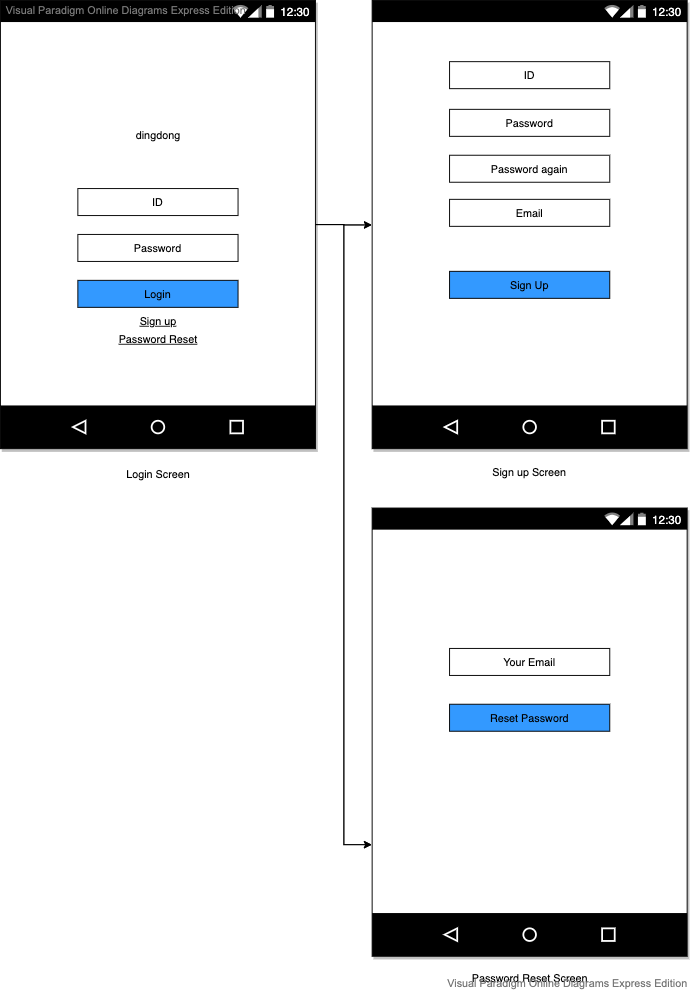
\includegraphics[width=6cm]{images/image0.png} 
\end{subfigure}
\begin{subfigure}
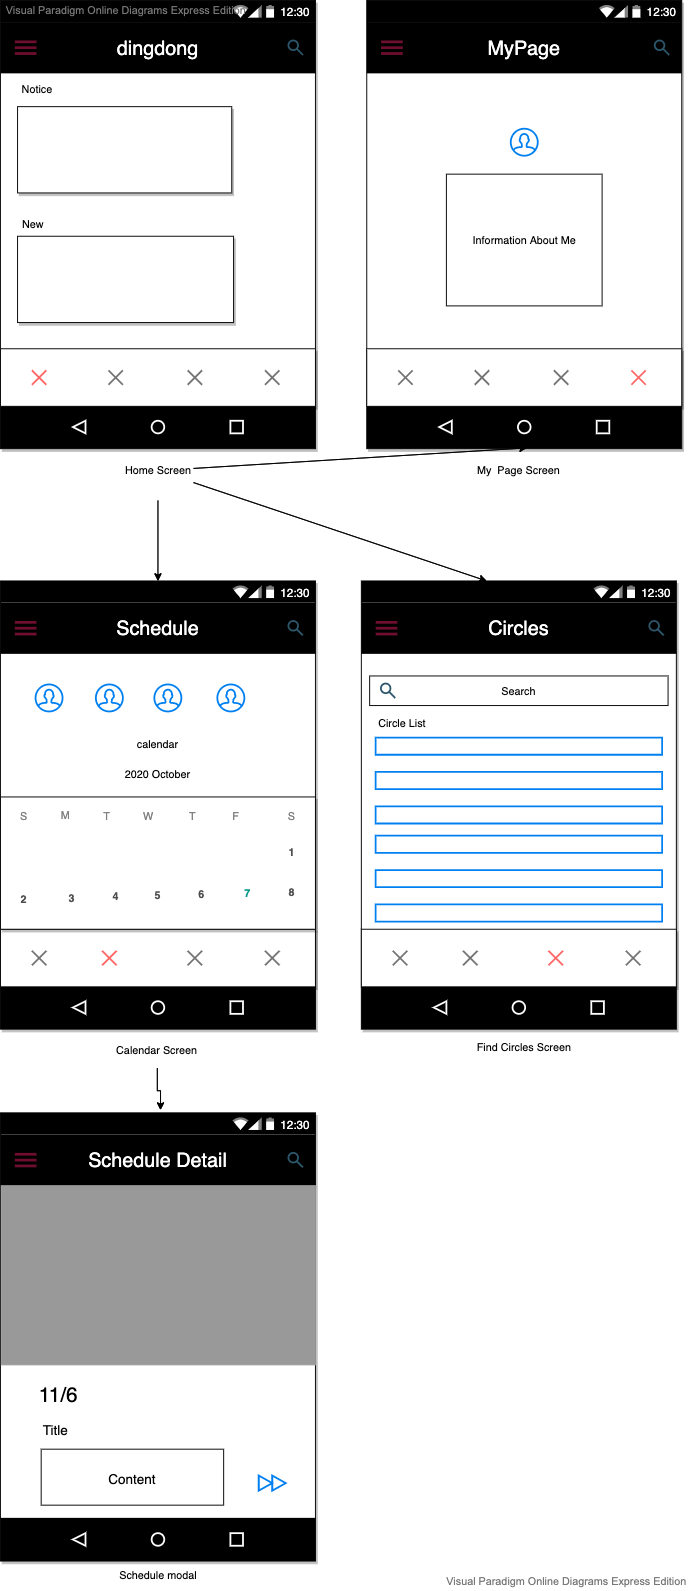
\includegraphics[width=6cm]{images/image3.png}
\end{subfigure}

\caption{Log In and Main Page}
\label{fig:image2}
\end{figure}

\begin{figure}[t]
    \centering
    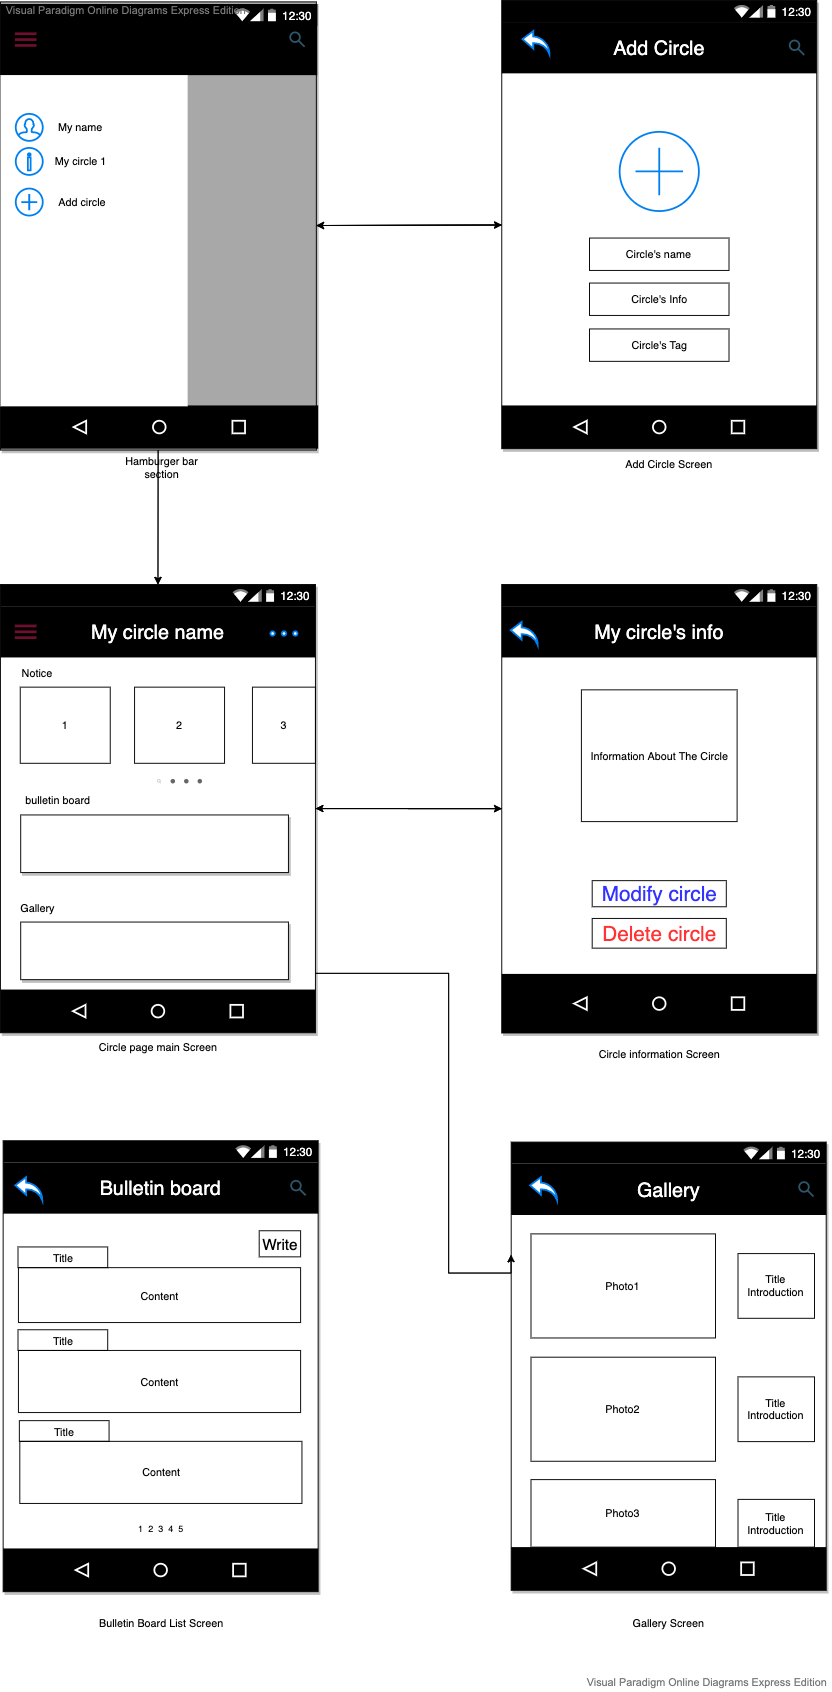
\includegraphics[width=8cm]{images/image8.png}
    \caption{Hamburger Bar Navigation}
    \label{fig: Views}
\end{figure}
\begin{figure}[b]
    \centering
    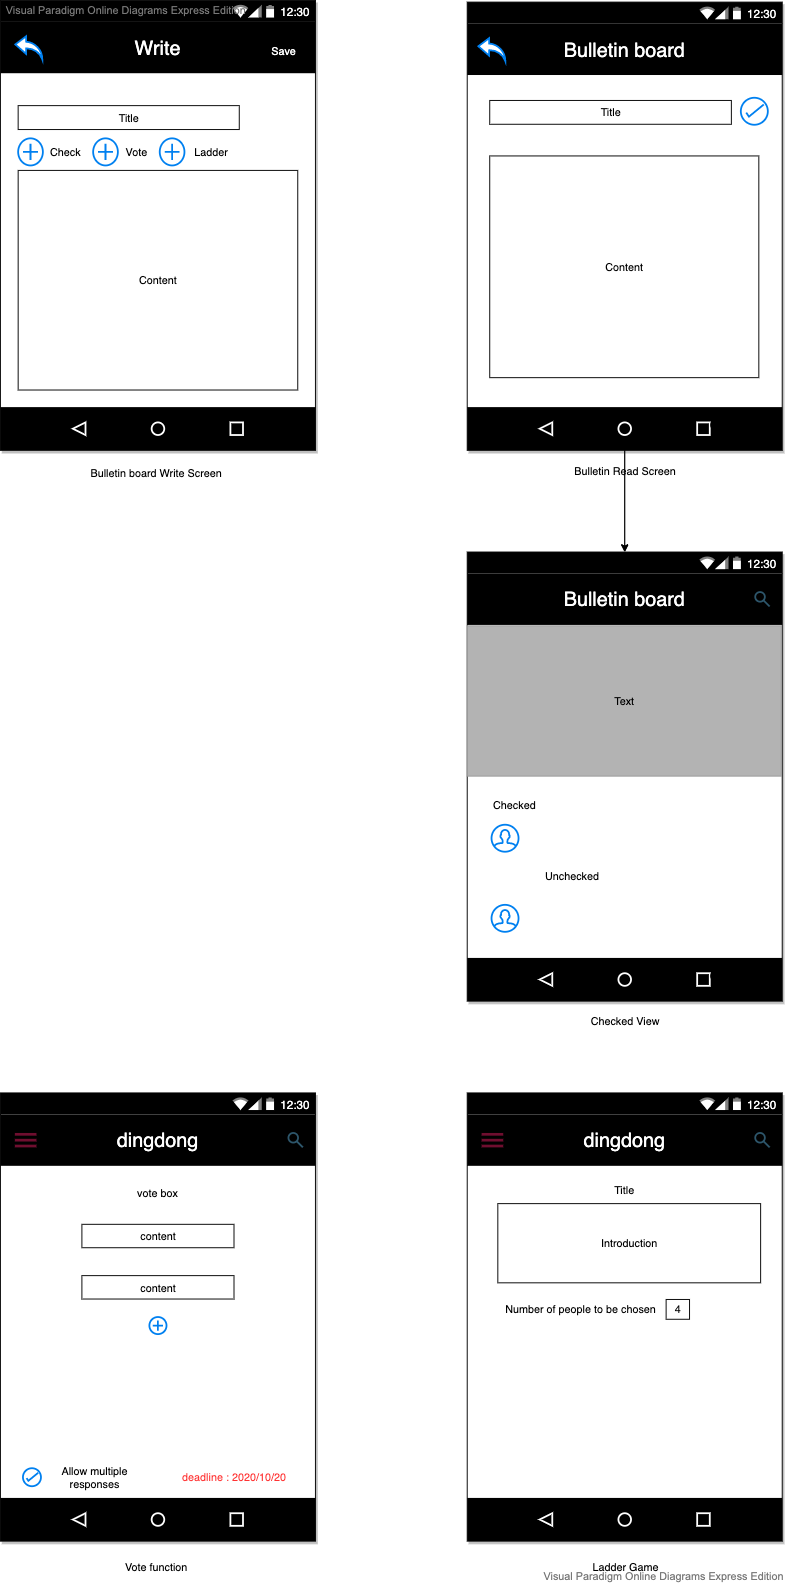
\includegraphics[width=8cm]{images/image9.png}
    \caption{Posting to a board}
    \label{fig: Views}
\end{figure}
\clearpage
\section{Overall Architecture}
\begin{figure}[h]
    \centering
    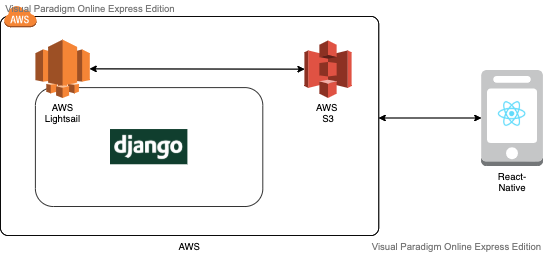
\includegraphics[width=8cm]{images/AWS.png}
    \caption{Overall Architecture}
    \label{fig:my_label}
\end{figure}
Figure4 explains our overall Architecture. On AWS, we used lighsail and s3. Lightsail is an easy-to-use cloud platform that offers useful services needed to build an application at very reasonable price. It was much easier to set up and use then ec2, which is the widely used service for computing. S3 was used for storing image files. User profile pictures, circle pictures are stored in the s3 bucket.
\subsection{Front-End Architecture}
For the front-end side, we used React-Native as our framework. So, the architecture of our app follows that of the React-Native. React-Native has components, which are separate items representing each views. Each components can be wrapped by or wrap other components, forming parent-child relationship. In Dingdong's front-end, the most-upper Component is App.tsx, wrapping other components inside it.
\begin{enumerate}
    \item One important aspect is Context. Context provides a way to pass data through the component tree without having to pass props down manually at every level. In other words, context is global variable that can be used all over the components, without having to be passed down from parent components.
    In our project, we used two Contexts. User and Circle. User context includes data about the user, including the username, circles he is involved in, and etc. Circle includes data for showing circle pages, such as bulletin board, posts and etc. These two data should be available in all components and thus are managed by context. In the figure below, the boxes that starts with 'I' represent interfaces. They define abstract design of the data. The contexts are User and Circle, which implements these interfaces in the data inside them. They also have functions inside which can be used to set the data.
    \begin{figure}[h]
        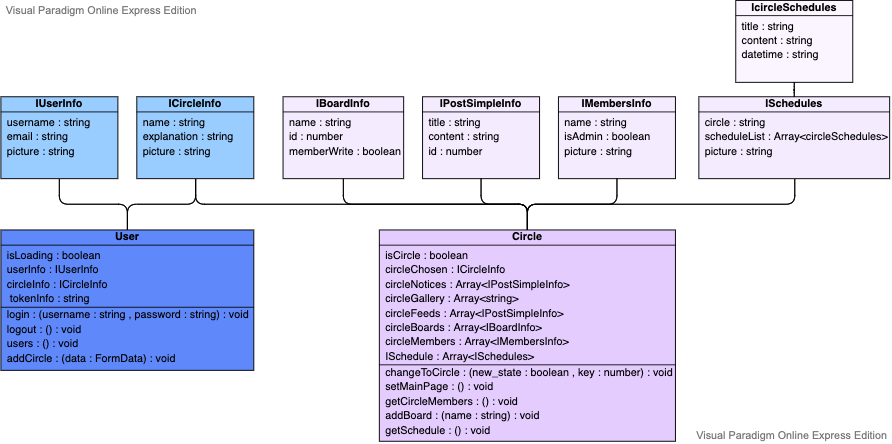
\includegraphics[width=9cm]{images/context.png}
        \caption{Context Structure}
        \label{fig: Views}
    \end{figure}
    \item The navigation architecture is as followed. First there is Tab Bar which can be used to navigate following screens: Home, Schedule, Circles, MyPage. In Home screen, there is a drawer, which allows navigation to each circle page, circle creation page, circle join page and if there are any new invitations to the circle that you are admin of, there will also be a button which navigate to respond screen. In each screens, there is stack navigation, which is a navigation that stacks new screens on top of the previous one. This is the most basic and widely used screen navigation in mobile apps. Figure 10 explains the whole navigation and a brief explanation of the screens used in our app.
\end{enumerate}
\subsection{Back-End Architecture}
For the back-end side, we follow the basic structure of Django framework. However, we also implemented django-restframework, which is slightly different to original django. In our back-end, we have 4 main components. models.py, serializers.py, urls.py, and views.py. Models.py is where we define models, the database structure that we use in the project. This is where we define users, circles, membership and etc. Each class members inside these model classes represent fields. These model classes are converted in to database tables by django. Serializers allow complex data such as querysets and model instances to be converted to native Python datatypes that can then be easily rendered into JSON, XML or other content types. These serializer classes are defined in serializers.py file. In urls.py, we defined urls paths which dispatches views for each paths. In views.py we defined each views for requests to the url paths we defined earlier. 
\begin{figure}[h]
    \centering
    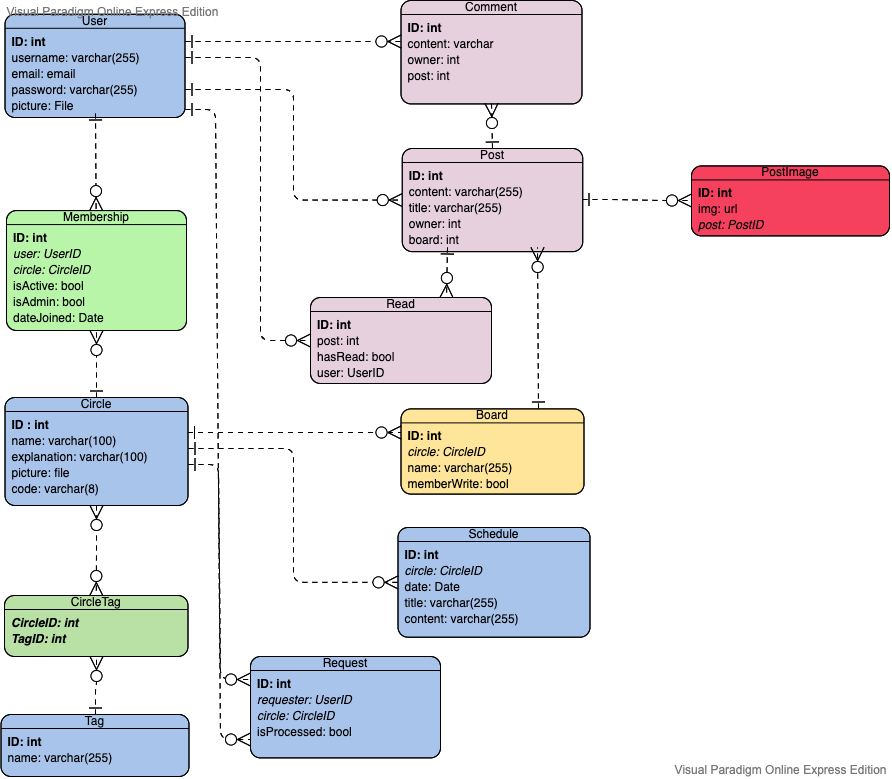
\includegraphics[width=8cm]{images/erd.png}
    \caption{ER Diagram}
    \label{fig:my_label}
\end{figure}
\clearpage
\subsection{Database Structure}
\begin{enumerate}
    \item User: The User table contains user data. We inherited Django's default user model to created our own model because we needed our users to have their own profile pictures.
    \item Circle:  Circle table contains data about circles. Each entry has name, explanation, unique code and picture.
    \item Membership: Membership table connects users and circles. It defines the membership status of user to a circle. Each entry explains whether the user is admin, is active and the date of join.
    \item Tag: Tag table contains tags that explains the circle. For instance, 'sports' is a type of tag that explains circles which are related o sports.
    \item CircleTag: CircleTag connects circles and tags.
    \item Board: Board table contains data of boards. The circle the board is in, name of the board and whether members are allowed to write to a board.
    \item Post: Post table contains data of each posts. The title, content, the board it is in, and the owner of the post.
    \item Comment: Comment table contains data of comments to a post.
    \item PostImage: PostImages contains data of pictures for posts. 
    \item Read: Read table contains whether the user has read the post of not.
    \item Schedule: Schedule table contains schedule data for circles.
    \item Request: Request table contains requests to join a circle. These requests are shown to the admins of a circle and they can process these requests either by accepting it or declining it.
\end{enumerate}
\begin{table}[t]
\caption{Api Document}
\begin{tabular}{|l|l|l|}
\hline
\textbf{Address}& \textbf{Method} & \textbf{Explanation}                                                                                       \\ \hline
ping                                                                                                                            & POST   & \begin{tabular}[c]{@{}l@{}}returns "pong". \\ To check if connected.\end{tabular}                  \\ \hline
signup                                                                                                                          & POST   & To signing up                                                                                      \\ \hline
login                                                                                                                           & POST   & To Login                                                                                           \\ \hline
user                                                                                                                            & GET    & \begin{tabular}[c]{@{}l@{}}To get information \\ about the user\end{tabular}                       \\ \hline
user/circles                                                                                                                    & GET    & \begin{tabular}[c]{@{}l@{}}To get information about \\ the circle user is a member of\end{tabular} \\ \hline
users/\textless{}username\textgreater{}                                                                                         & GET    & \begin{tabular}[c]{@{}l@{}}To get information \\ about other users\end{tabular}                    \\ \hline
membership                                                                                                                      & POST   & To join a circle                                                                                   \\ \hline
membership                                                                                                                      & DELETE & To withdraw from a circle                                                                          \\ \hline
circles                                                                                                                         & POST   & To create a circle                                                                                 \\ \hline
circles                                                                                                                         & GET    & To get list of circles                                                                             \\ \hline
circles                                                                                                                         & DELETE & To remove a circle                                                                                 \\ \hline
circles/\textless{}circle\_name\textgreater{}                                                                                   & GET    & \begin{tabular}[c]{@{}l@{}}To get information \\ about a circle\end{tabular}                       \\ \hline
\begin{tabular}[c]{@{}l@{}}circles/\textless{}circle\_name\textgreater\\ /members\end{tabular}                                  & GET    & To get members of a circle                                                                         \\ \hline
\begin{tabular}[c]{@{}l@{}}circles/\textless{}circle\_name\textgreater\\ /boards\end{tabular}                                   & GET    & To get list of boards in a circle                                                                  \\ \hline
\begin{tabular}[c]{@{}l@{}}circles/\textless{}circle\_name\textgreater\\ /boards\end{tabular}                                   & POST   & To create a board for a circle                                                                     \\ \hline
\begin{tabular}[c]{@{}l@{}}circles/\textless{}circle\_name\textgreater\\ /notices\end{tabular}                                  & GET    & To get list of notices of a circle                                                                 \\ \hline
board/\textless{}board\_id\textgreater{}                                                                                        & GET    & To get information of a board                                                                      \\ \hline
board/\textless{}board\_id\textgreater{}                                                                                        & PUT    & To modify a board                                                                                  \\ \hline
board/\textless{}board\_id\textgreater{}/post                                                                                   & POST   & To create a post in a board                                                                        \\ \hline
board/\textless{}board\_id\textgreater{}/post                                                                                   & GET    & To get posts inside a board                                                                        \\ \hline
post/\textless{}board\_id\textgreater{}/read                                                                                    & POST   & To mark 'read' to a post                                                                           \\ \hline
post/\textless{}board\_id\textgreater{}/comment                                                                                 & POST   & To create a comment to a post                                                                      \\ \hline
post/\textless{}board\_id\textgreater{}/comment                                                                                 & GET    & To get comment list of a post                                                                      \\ \hline
\begin{tabular}[c]{@{}l@{}}post/\textless{}board\_id\textgreater{}/comment\\ /\textless{}comment\_id\textgreater{}\end{tabular} & DELETE & To delete a comment                                                                                \\ \hline
\begin{tabular}[c]{@{}l@{}}post/\textless{}board\_id\textgreater{}/comment\\ /\textless{}comment\_id\textgreater{}\end{tabular} & PUT    & To modify comment                                                                                  \\ \hline
schedules                                                                                                                       & GET    & To get schedules of circle                                                                         \\ \hline
schedules                                                                                                                       & POST   & To create a schedule for a cicle                                                                   \\ \hline
\end{tabular}
\end{table}
\subsection{Api Document}
Table 2 explains the Apis that we used for this project. We tried to keep our api as RESTFUL as possible, simplifying our api addresses and following the RESTFUL API architectural style.


\section{Directory Organization}
\begin{table}[htbp]
\centering


\caption{Frontend Directory}
\begin{tabular}{|l|l|l|}
\hline
Directory     &File names
            & Module \\
\hline
/src                 
& App.tsx                                                       
& Main Dir      \\ 
\hline
/src/Api                 
& Api.js, Config.js                                                        & Api Dir      \\ 
\hline
/src/Asset/Images                
& [...Images].png                                                        & Asset Dir      \\
\hline
/src/Components              
& \begin{tabular}[c]{@{}l@{}}/Bubbles/index.tsx\\ /Button/index.tsx\\ /IconButton/index.tsx\\ /ImageButton/index.tsx\\ /Input/index.tsx\\ /Loading/index.tsx\\ /NewsBox/index.tsx\\ /NoticeBox/index.tsx\\ /Tab/index.tsx\end{tabular}                                                        & Component Dir      \\
\hline
/src/Constants                
& Constants.tsx                                                       
& Constant Dir     \\ 
\hline
/src/Context                  
& \begin{tabular}[c]{@{}l@{}}/Circle/index.tsx\\ /Circle/@type/index.d.ts\\ User/index.tsx\\ User/@type/index.d.ts\end{tabular}                                                       
& Context Dir       \\ 
\hline
/src/Screen                
& \begin{tabular}[c]{@{}l@{}}Navigator.tsx\\ /@type/index.d.ts\\ /AddBoard/index.tsx\\ /AddCircle/index.tsx\\ /BulleteinBoard/index.tsx\\ /Calendar/index.tsx\\ /CirclePageEdit/index.tsx\\ /Circles/index.tsx\\ /Drawer/index.tsx\\ /Gallery/index.tsx\\ /Home/index.tsx\\ /Information/index.tsx\\ /Login/index.tsx\\ /MyCircle/index.tsx\\ /MyPageEdit/index.tsx\\ /MyPage/index.tsx\\ /Onboarding/index.tsx\\ /PasswordReset/index.tsx\\ /Read/index.tsx\\ /Signup/index.tsx\\ /Write/index.tsx\end{tabular}                                                       
& Screen Dir      \\ 
\hline
\end{tabular}
\end{table}



\begin{table}[htbp]
\centering
\caption{Backend Direcotry}
\begin{tabular}{|l|l|l|} 
\hline
Directory          & File names                                                                                                & Module~    \\ 

\hline
/                  & manage.py, db.sqlite3, aws.py                                                                            & Main Dir       \\ 

\hline
/dingdong/settings & base.py, local.py, prod.py~                                                                               & Setting Dir       \\ 
\hline
/circle            & \begin{tabular}[c]{@{}l@{}}admin.py, apps.py, models.py, \\serializers.py, urls.py, views.py\end{tabular} & Circle Dir     \\
\hline
\end{tabular}
\end{table}
\subsection{Front End Structure}
\begin{enumerate}
    \item Main Dir: App.tsx is a typescript file which is the main file that will be executed at the very first time.
    \item Api Dir: This is where we keep api functions that we need in the app to communicate with the server. Config.js file is where the api base address and base functions for sending http request are located. Api.js file is where we keep all functions that we use in the app.
    \item Asset Dir: Asset directory keeps all static files. For now, only images are the files that we need. These images include all icons used in the app , splash screen image and so on.
    \item Component Dir: This is where we keep all the components that we use in the app. They are reusable components which are continuously used in the app. For instance, Input components are reused in many screens where inputs from user are needed.
    \item Constant Dir: This is where we keep the constants that we need. Most of the constants are related to the design, such as RGB code for the colors that we use in the app. Managing them as constants help to change the color at once and keep unity. For instance, we keep the RGB code for our main color, which is \#5F89FA. When we need to change the color, we can simply change it here instead of changing in every file that we used this color.
    \item Context Dir: This is where we keep the Context data. In React (and React Native), Context provides a way to pass data through the component tree without having to pass props down manually at every level. Thus, we keep the important and diversely used data in Context. These data are the circle information and the user information. Each of these files also has methods to set these data.
    \item Screen Dir: This is where we keep the Screens. Screens are views that will be displayed on the app. Each screen file has its class and rendering functions to display views.
\end{enumerate}
\subsection{Back End Structure}
\begin{enumerate}
    \item Main directory: Main directory. manage.py is the file that help to manage the project. db.sqlite3 is the database and aws.py is where we keep the aws file passwords.
    \item Setting directory: This is where we settings for the project. base.py has the base class settings that we need. local.py and prod.py inherit the base class and have different settings for local server and production server.
    \item Circle directory: Where we keep all views, urls and models needed for the project. models.py has all database models that we need, such as user Table, circle table and so on. urls.py has urls that will each be mapped to views. views.py has functions that will be called for each request to the url.
\end{enumerate}
\begin{figure}[h]
    \centering
    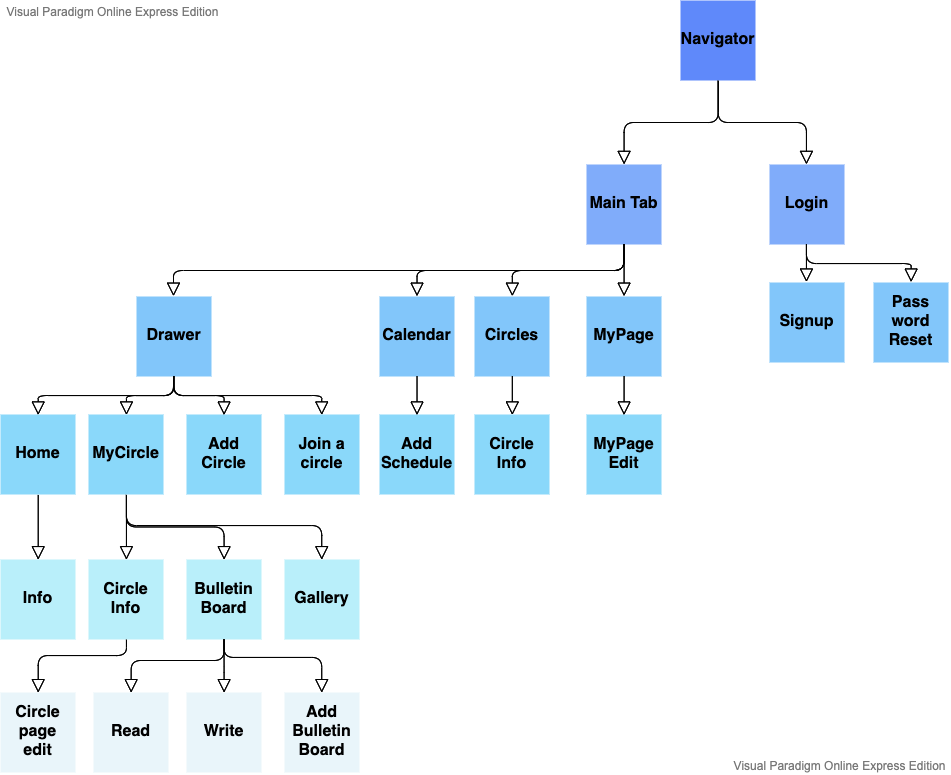
\includegraphics[width=8cm]{images/navigation3.png}
    \caption{Navigation Structure}
    \label{fig:my_label}
\end{figure}
\clearpage

\section{Use cases}
\begin{enumerate}
    \begin{figure}[h]
        \centering
        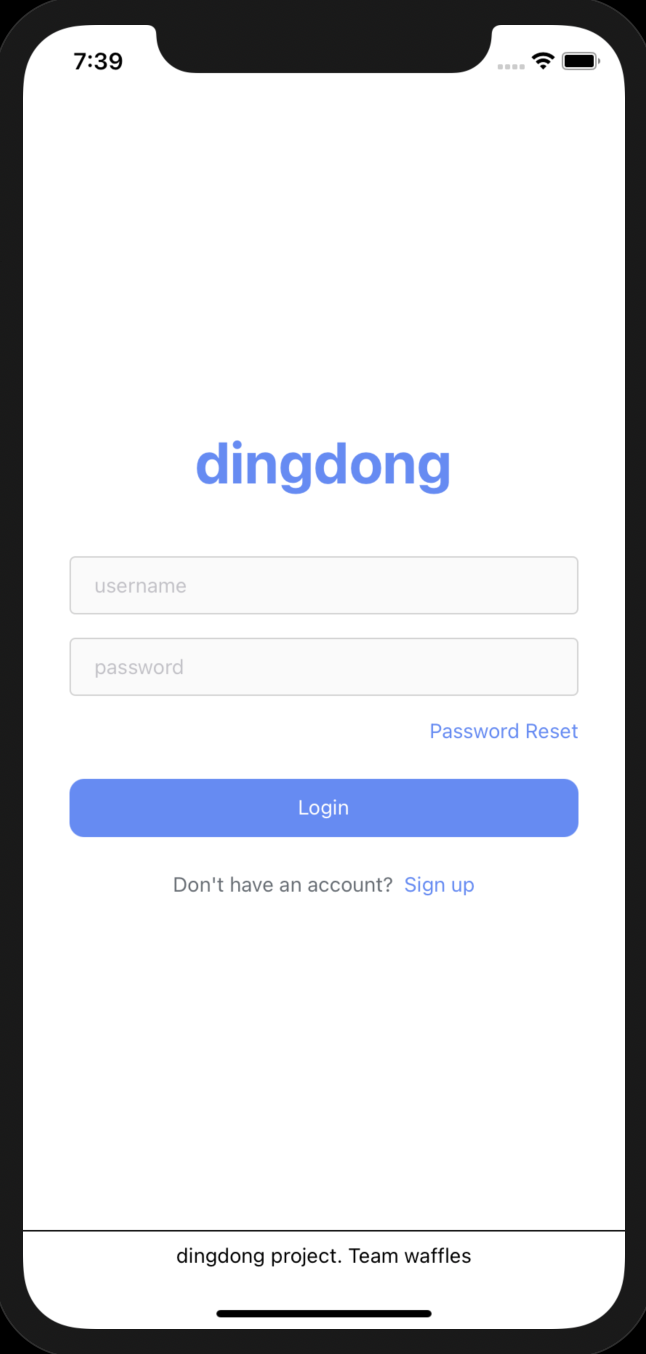
\includegraphics[width=4cm]{images/login.png}
        \caption{Login Screen}
        \label{fig:my_label}
    \end{figure}
    \item Login Screen: The first screen to be shown to user when user starts the app for the first time. The username and passwords are required to login. Pressing login button will navigate to main screen on success and alert 'wrong user information' on fail. Pressing on Password Rest will navigate to Password Reset screen. Pressing on Sign up will navigate to Sign up screen.
    \begin{figure}[h]
        \centering
        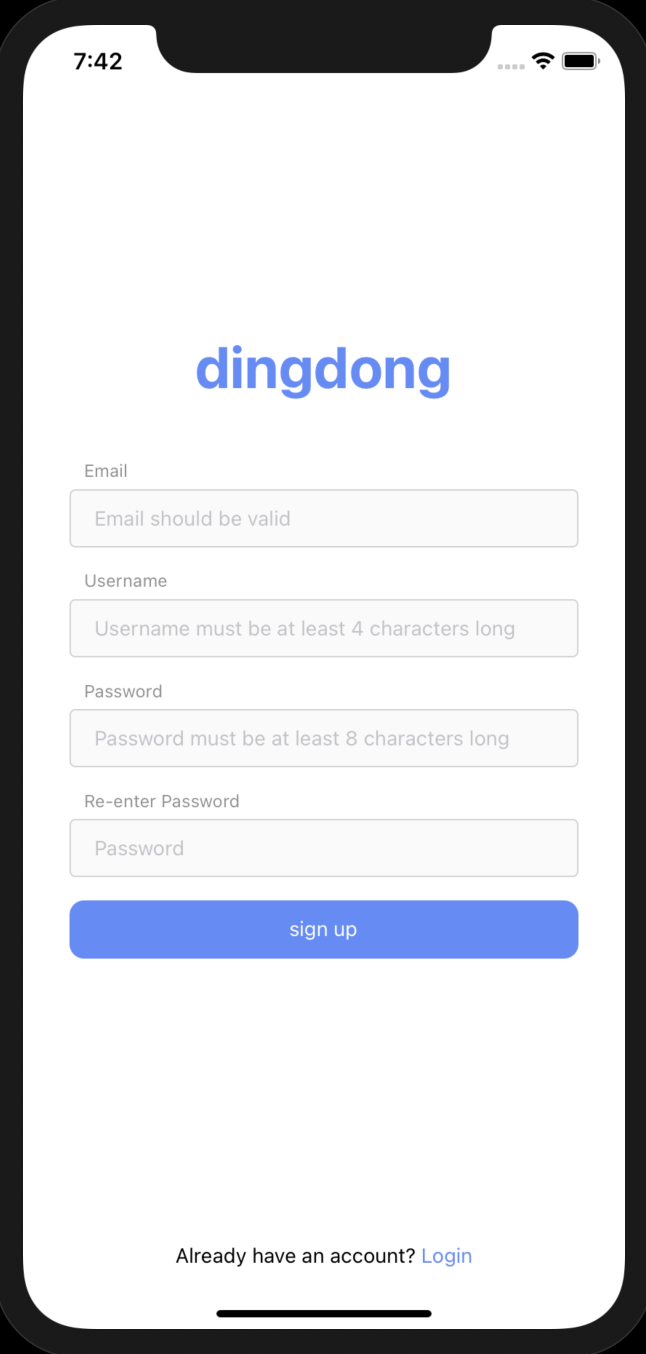
\includegraphics[width=4cm]{images/signup.png}
        \caption{Sign Up Screen}
        \label{fig:my_label}
    \end{figure}
    \item Sign Up Screen: The sign up screen has four input forms and sign up button. Email should match the email regular expression. Username must be between 4 and 20 characters. Password must be between 8 to 50 characters. Re-enter password must match the password. If Sign up succeed, it will navigate to the login screen, and if it fail, it will alert that sign up has failed.
    \begin{figure}[h]
        \centering
        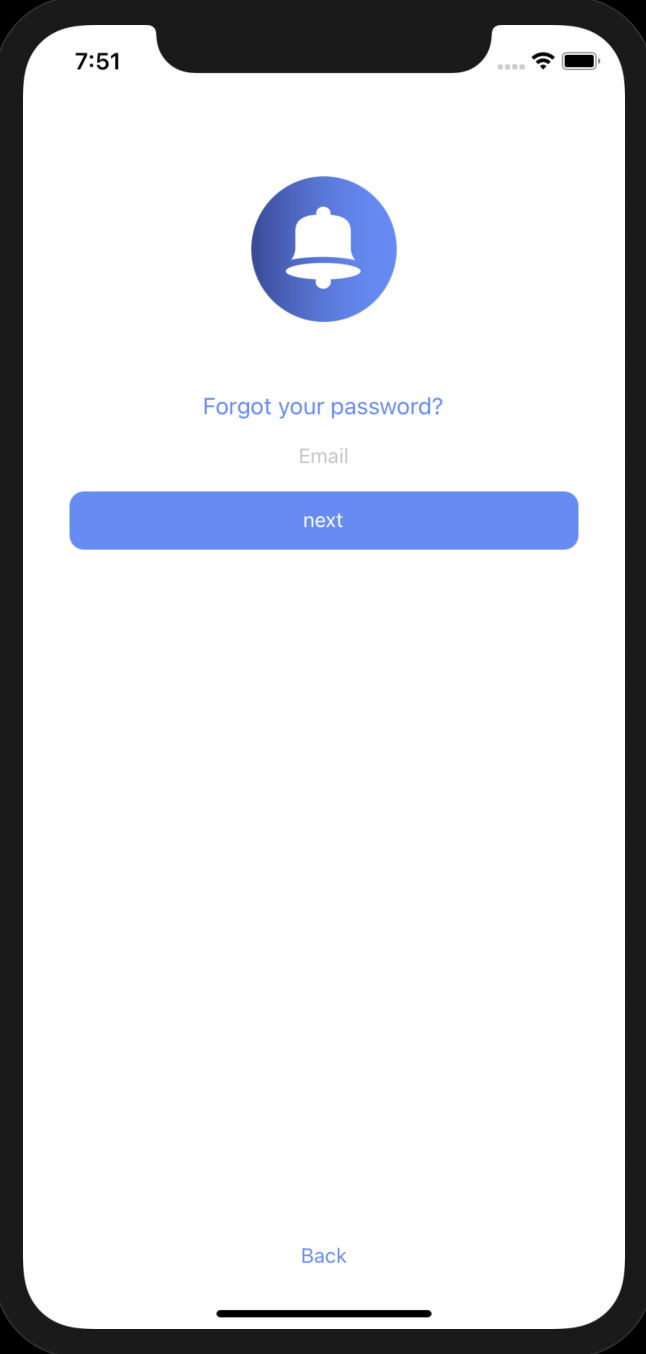
\includegraphics[width=4cm]{images/passwordreset.png}
        \caption{Password Reset Screen}
        \label{fig:my_label}
    \end{figure}
    \item Password Reset Screen: To reset, password, the email address is needed. If the email address is correct, the link to change the password will be sent to the email.
    \begin{figure}[h]
        \centering
        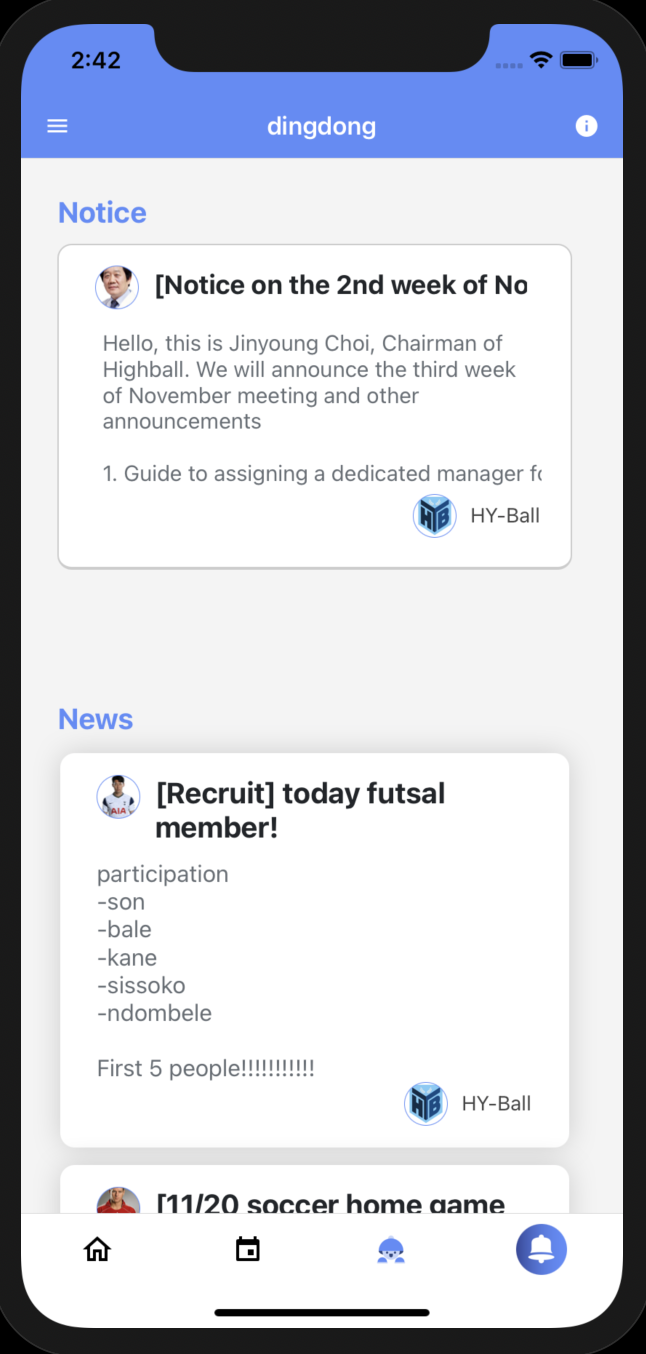
\includegraphics[width=4cm]{images/home.png}
        \caption{Home Screen}
        \label{fig:my_label}
    \end{figure}
    \item Home Screen: The main screen is the first screen after login, or after starting the app with tokens stored in the storage. In the header, pressing the hamburger icon will show the drawer screen. The information icon on the right side will navigate to information screen of the app.
    The Notice box is where we display the latest notices from all the circles the use joined. Maximum 5 notices will be shown. Pressing on each will navigate to the Post Read Screen. The News box is where we display all posts from all circles. Pressing on each will navigate to the Post Read Screen.
    \begin{figure}[h]
        \centering
        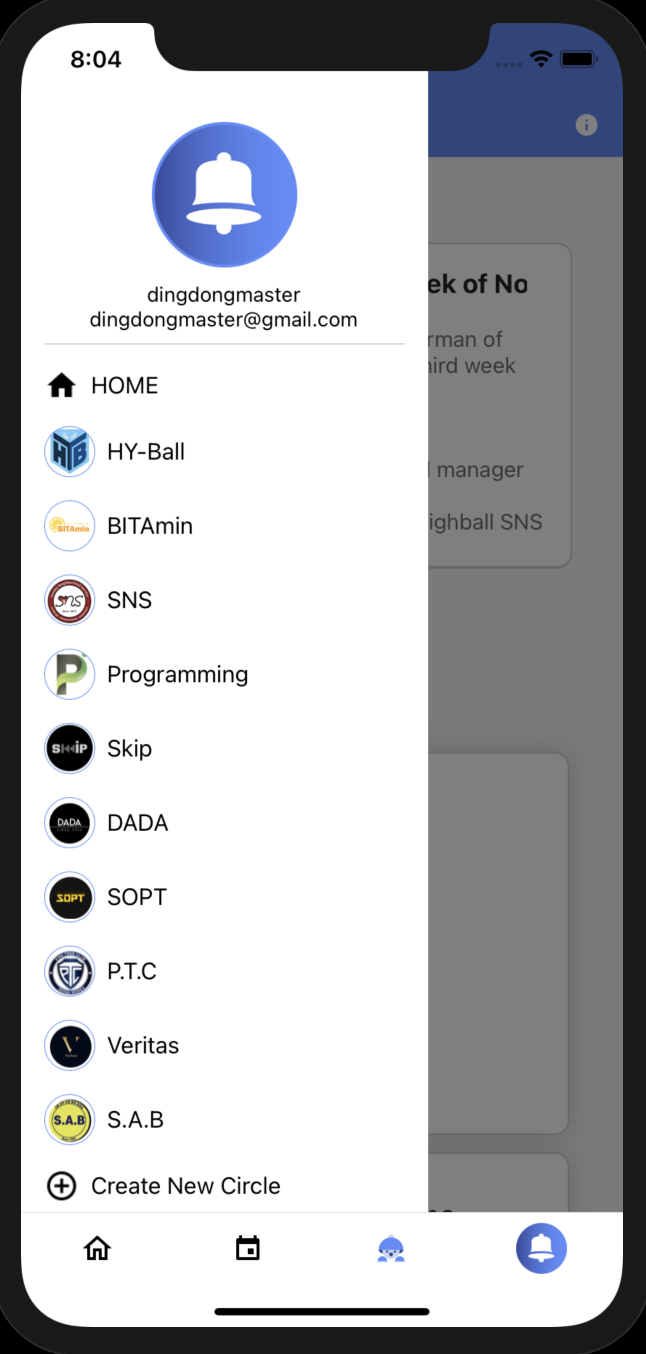
\includegraphics[width=4cm]{images/drawer1.png}
        \caption{Drawer Info and Circles Screen}
        \label{fig:my_label}
    \end{figure}
    \begin{figure}[h]
        \centering
        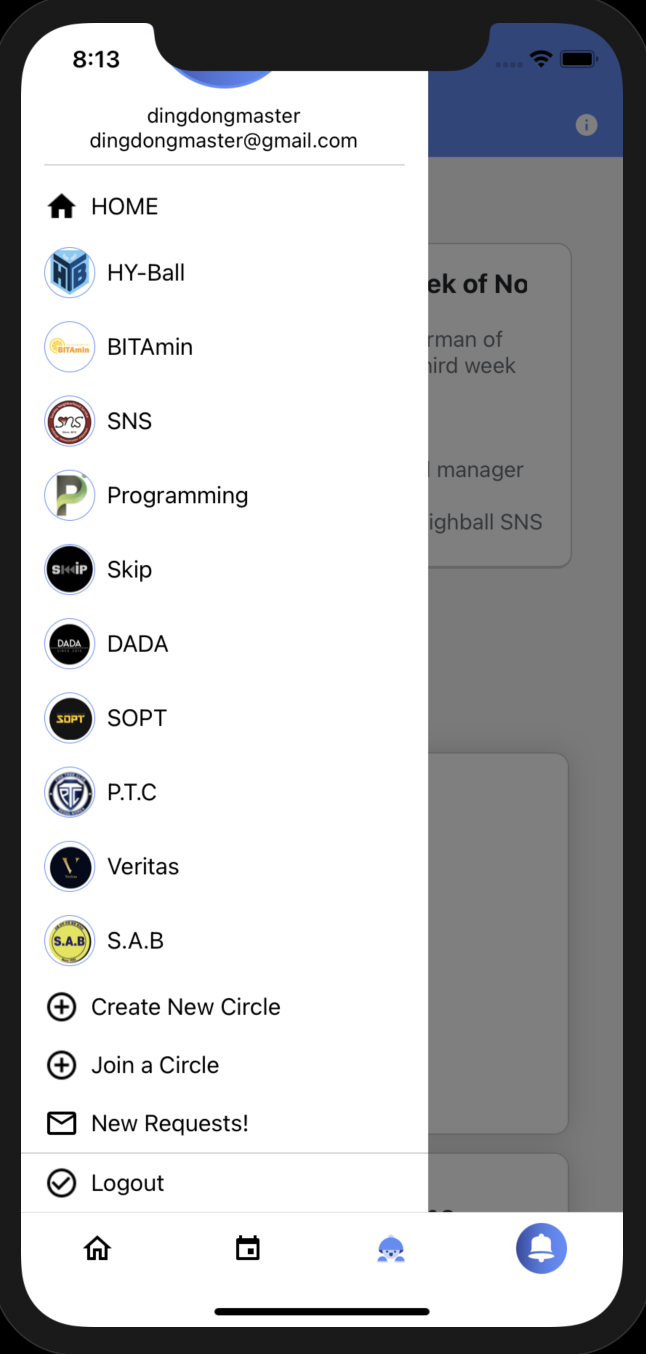
\includegraphics[width=4cm]{images/drawer2.png}
        \caption{Drawer Etc Screen}
        \label{fig:my_label}
    \end{figure}
    \item Drawer Screen: Drawer screen display user information, list of circles that the use has joined, and several buttons. In the circle list, pressing on each will navigate to circle page. Beneath the list, Create new circle and join a circle button is located. When there are new requests to join a circle that the user is admin of, the ``New Requests!" button will be shown, which will navigate to request list page on press. At the bottom, the log out button is located. Pressing the button will log out and navigate to the login screen.
    \begin{figure}[h]
        \centering
        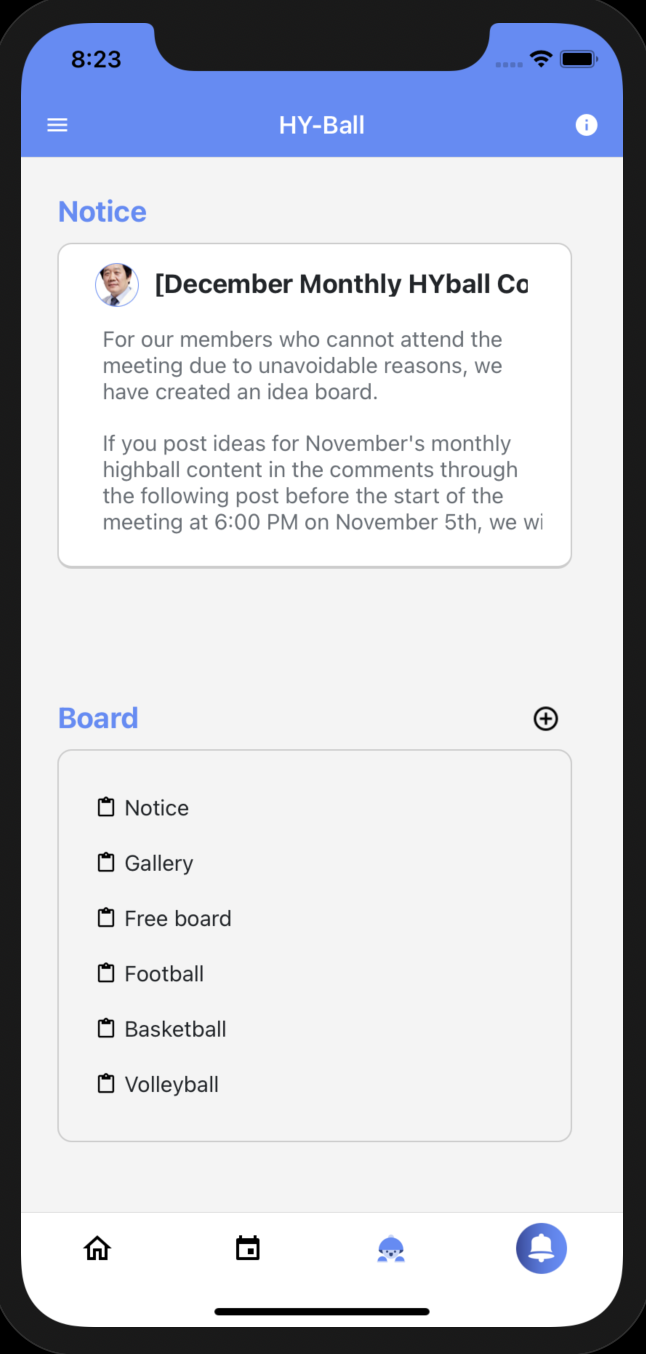
\includegraphics[width=4cm]{images/circlehome.png}
        \caption{Circle Home Top Screen}
        \label{fig:my_label}
    \end{figure}
    \begin{figure}[h]
        \centering
        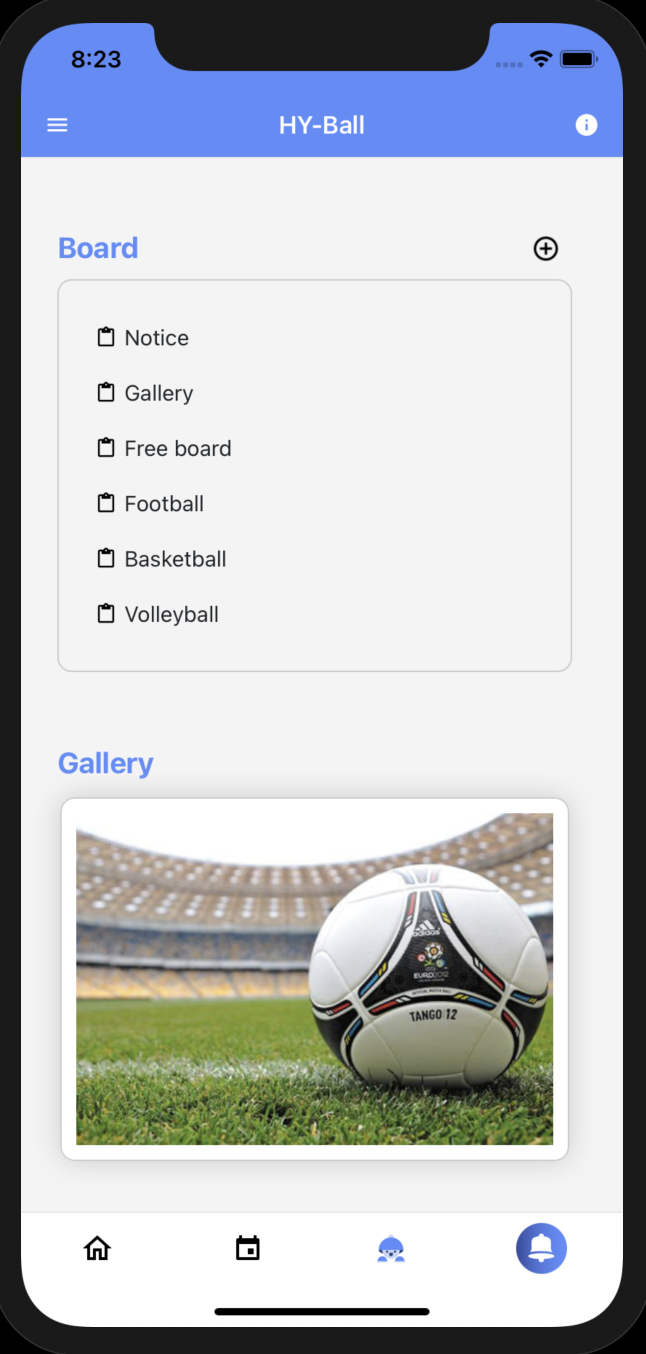
\includegraphics[width=4cm]{images/circlehome2.png}
        \caption{Circle Home Bottom Screen}
        \label{fig:my_label}
    \end{figure}
    \item Circle Screen: Circle screen is the main screen for each of the circles. The Notice box is similar to that of the main screen, but only displays notices of that specific circle. Th Board box shows list of boards created. Pressing on each will navigate to the Board screen. Pressing the plus button on the top-right will navigate to Board Create screen. Below the board list, there is the Gallery box which displays latest images posted on the gallery screen. Pressing on the information icon on the right side of the header will navigate to the information screen.
    \begin{figure}[h]
        \centering
        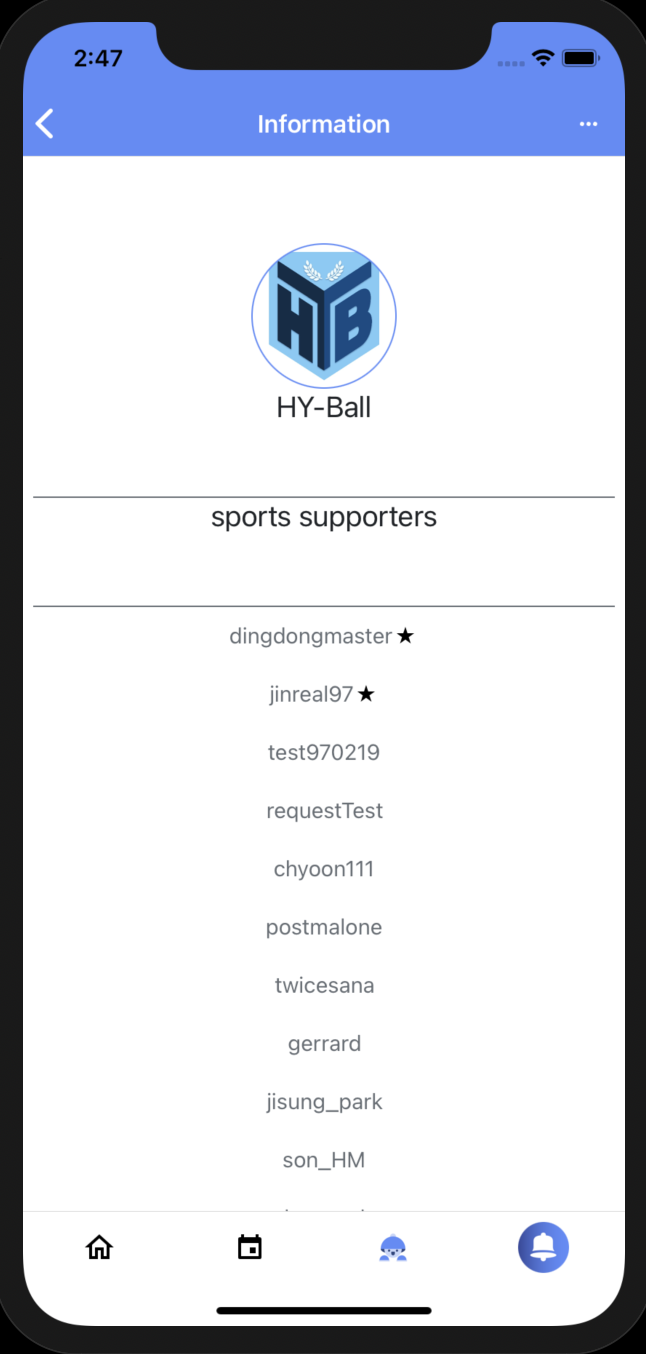
\includegraphics[width=4cm]{images/circleinformation1.png}
        \caption{Circle Information Screen}
        \label{fig:my_label}
    \end{figure}
    \begin{figure}[h]
        \centering
        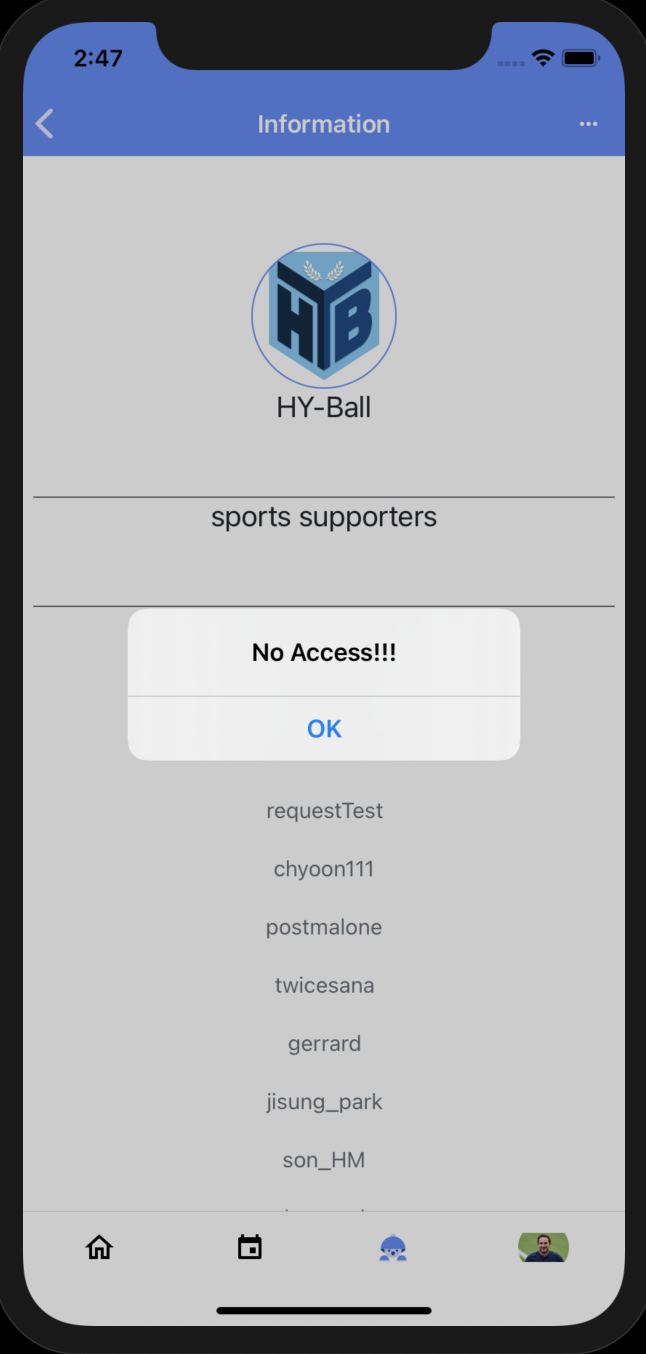
\includegraphics[width=4cm]{images/circleinformation2.png}
        \caption{Circle Information Access Edit Screen}
        \label{fig:my_label}
    \end{figure}
    \item Circle Information Screen: Circle information screen displays the name, the explanation and the members of the circle. A star on next to the name of the member signs the administrator. Pressing on the edit button on the right side of the header will navigate to the circle edit screen. Only admin of the circle are allowed to edit. If a non-admin user presses this button, it will alert "No Access".
    \begin{figure}[h]
        \centering
        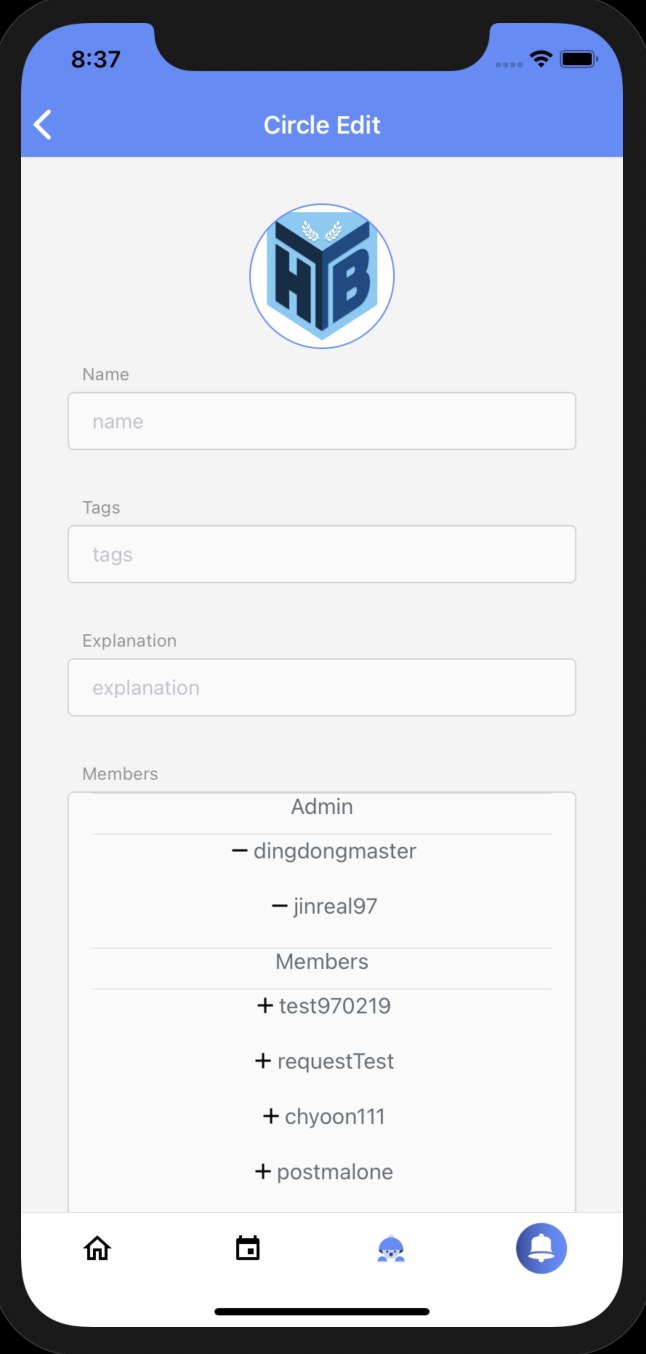
\includegraphics[width=4cm]{images/circleedit1.png}
        \caption{Circle Edit Screen}
        \label{fig:my_label}
    \end{figure}
    \begin{figure}[h]
        \centering
        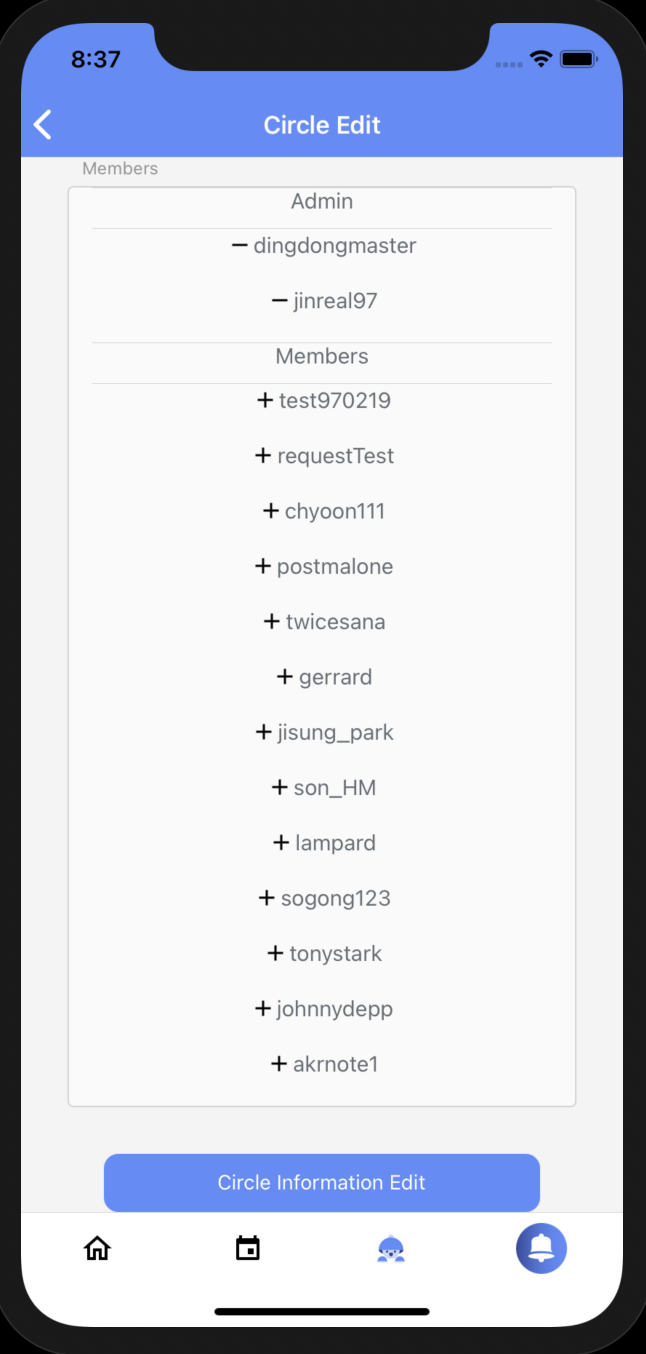
\includegraphics[width=4cm]{images/circleedit2.png}
        \caption{Circle Edit Members Screen}
        \label{fig:my_label}
    \end{figure}
    \item Circle Edit Screen: In the circle edit screen, user can change the name, tag, explanation and members-admin of the circle.
    \begin{figure}[h]
        \centering
        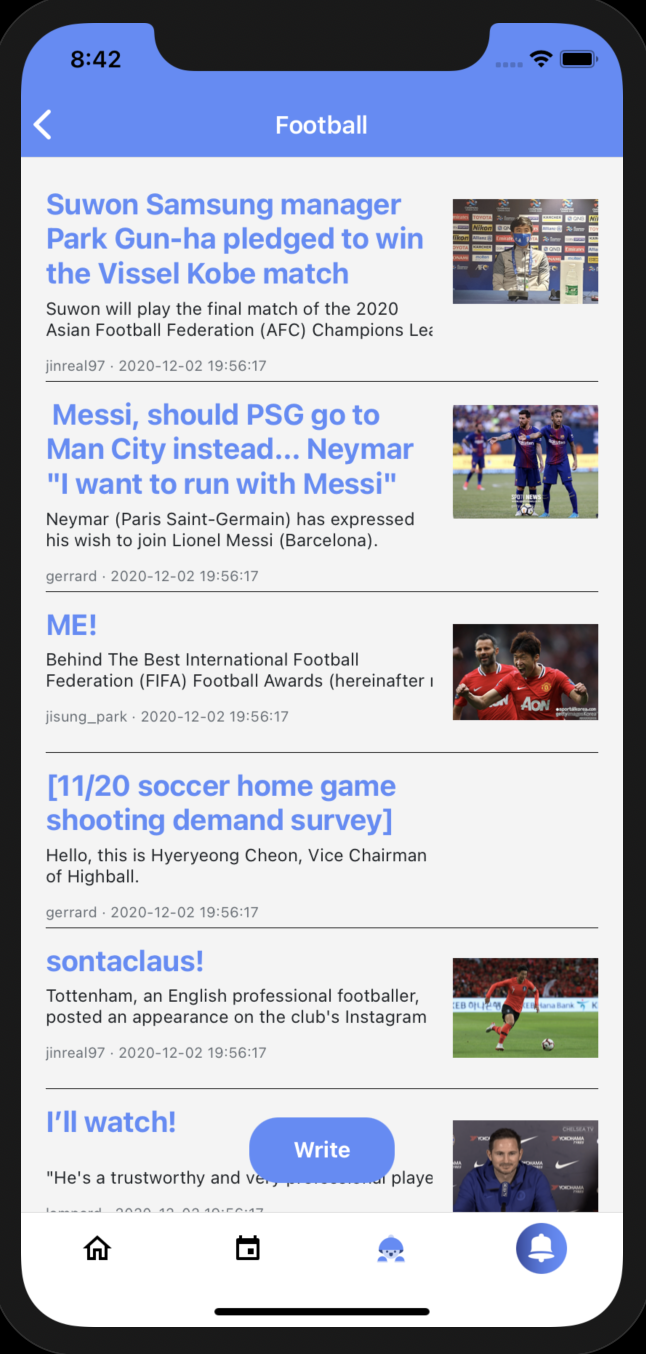
\includegraphics[width=4cm]{images/board.png}
        \caption{Circle Board Screen}
        \label{fig:my_label}
    \end{figure}
    \item Board Screen: In Board Screen, post list is shown. Pressing on each will navigate to the post read screen. Each item in the list displays the title, content, image(if there is any) and the user and creation time of the post. On the bottom of the screen, there is a write button which will navigate to post write screen.
    \begin{figure}[h]
        \centering
        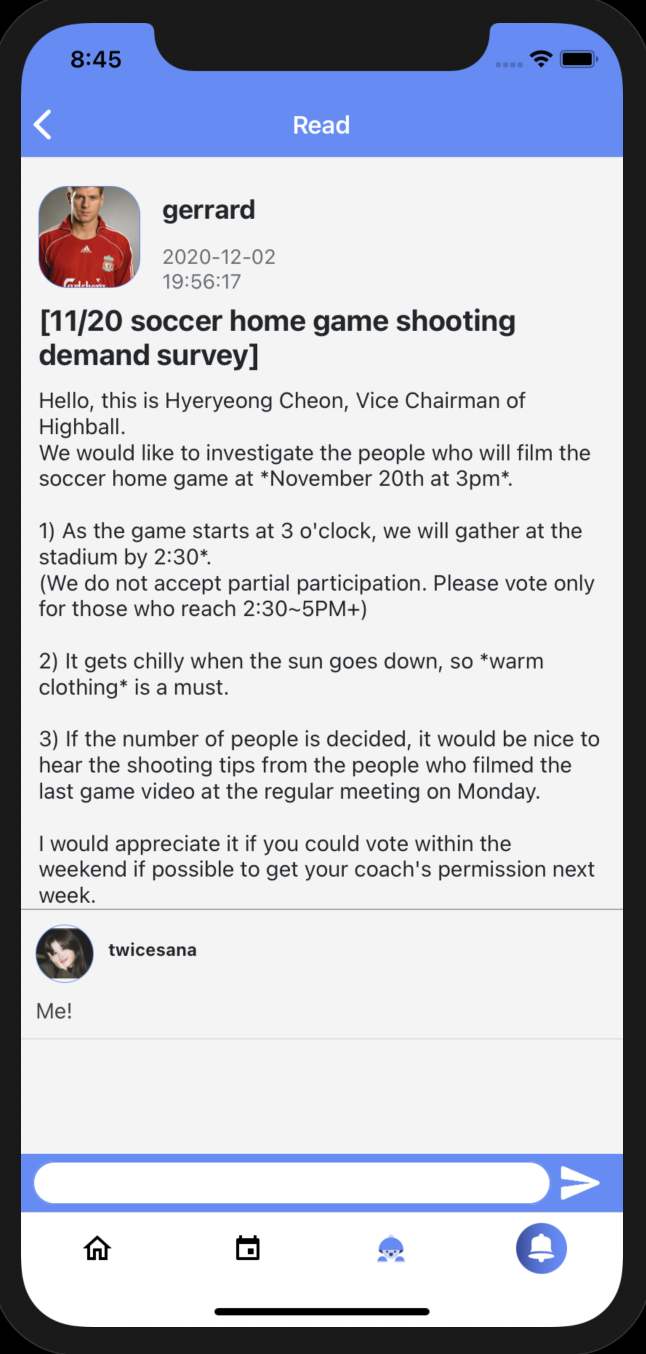
\includegraphics[width=4cm]{images/read1.png}
        \caption{Read Screen}
        \label{fig:my_label}
    \end{figure}
    \begin{figure}[h]
        \centering
        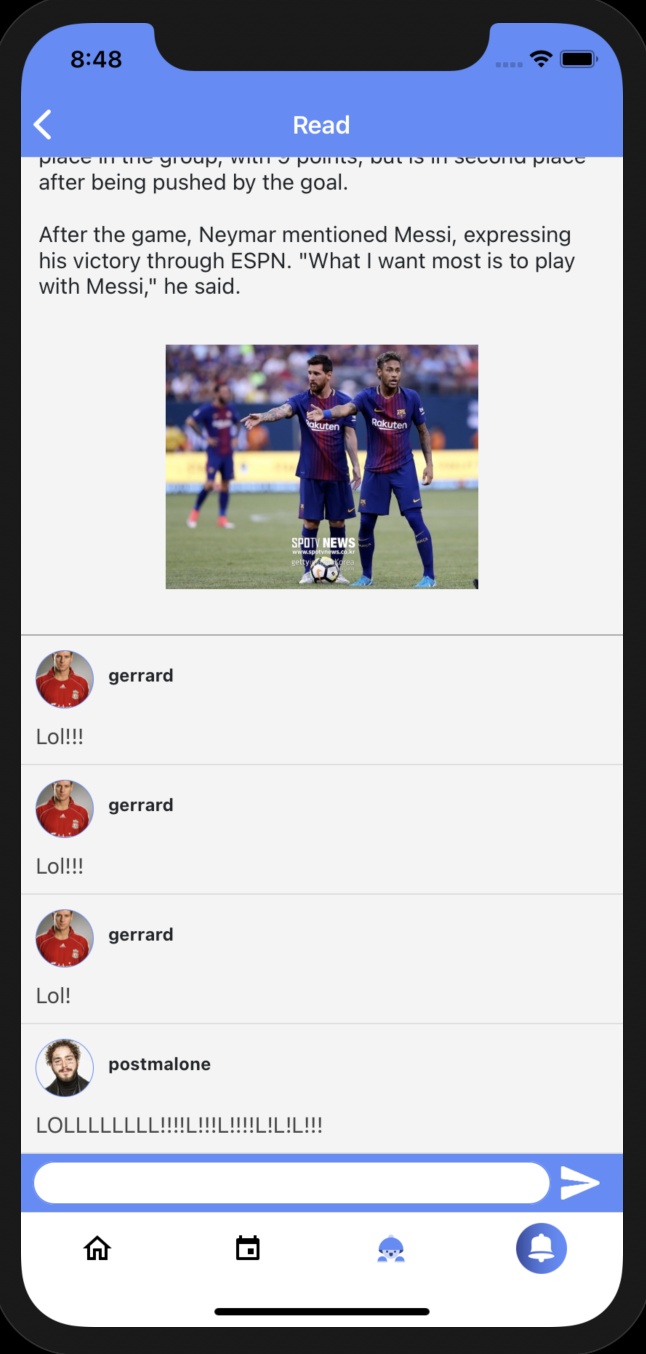
\includegraphics[width=4cm]{images/read2.png}
        \caption{Read Comment Screen}
        \label{fig:my_label}
    \end{figure}
    \begin{figure}[h]
        \centering
        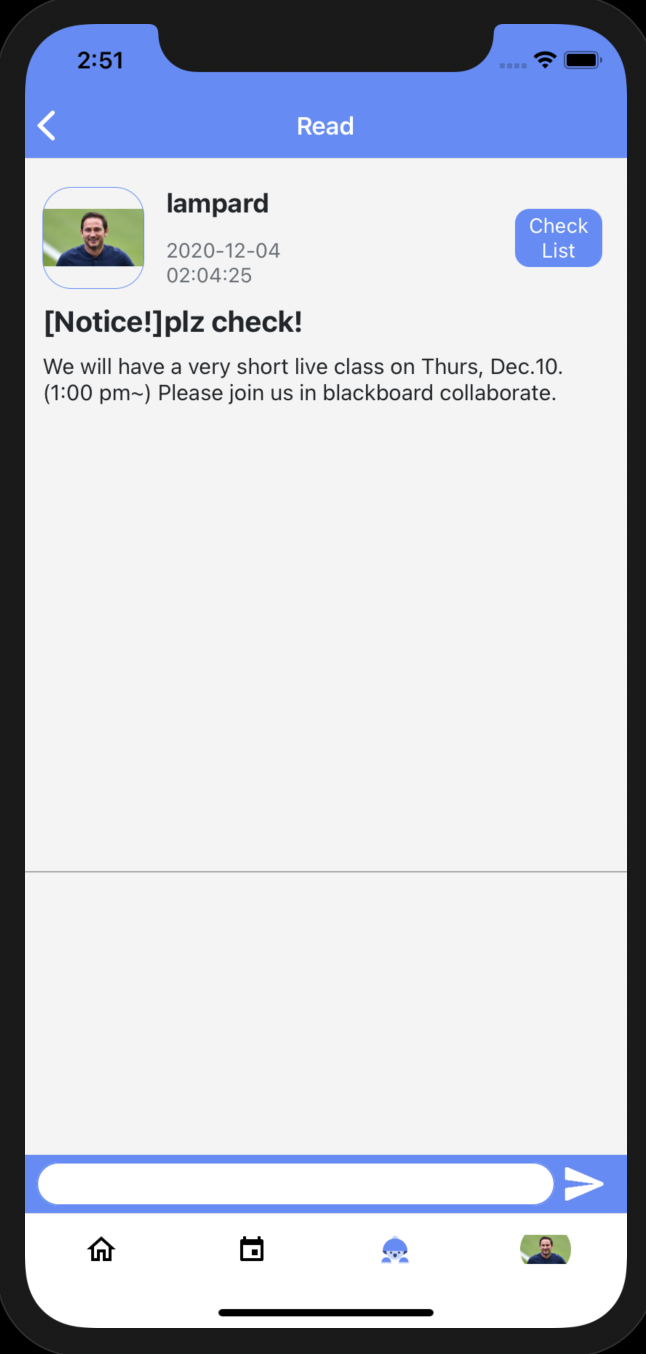
\includegraphics[width=4cm]{images/read3.png}
        \caption{Read Owner Check List Screen}
        \label{fig:my_label}
    \end{figure}
    \begin{figure}[h]
        \centering
        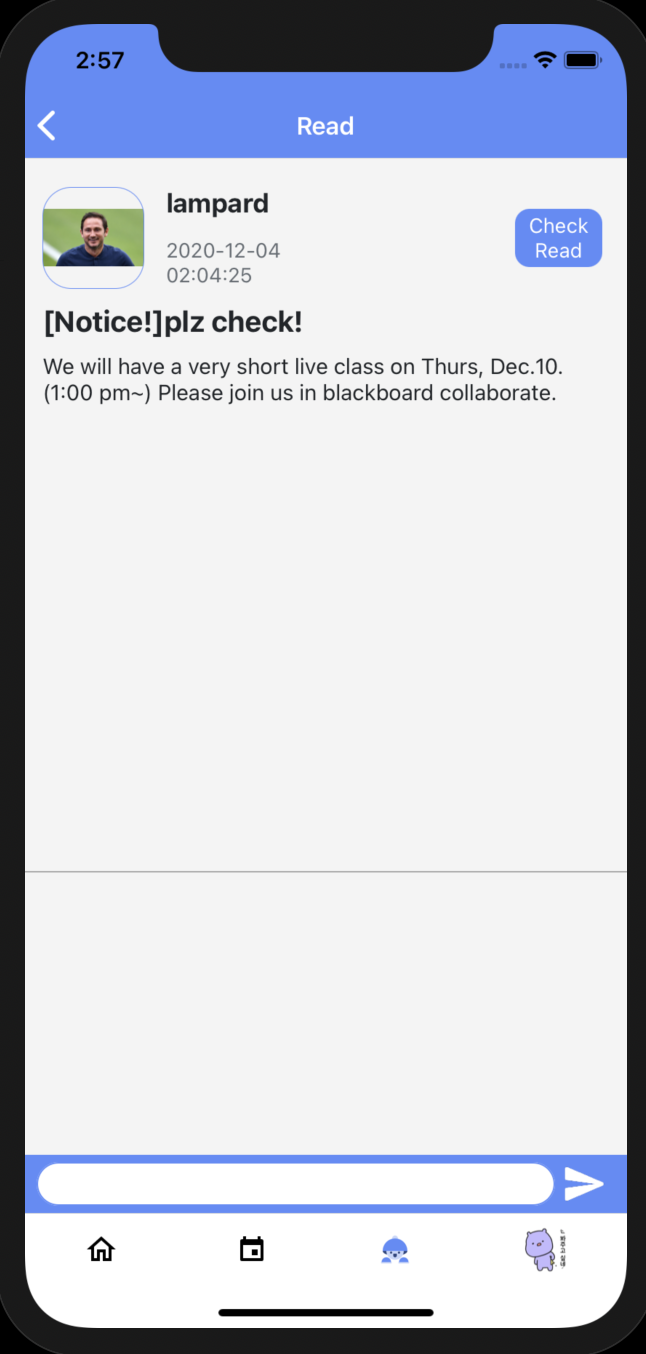
\includegraphics[width=4cm]{images/read4.png}
        \caption{Read Check Screen}
        \label{fig:my_label}
    \end{figure}
    \begin{figure}[h]
        \centering
        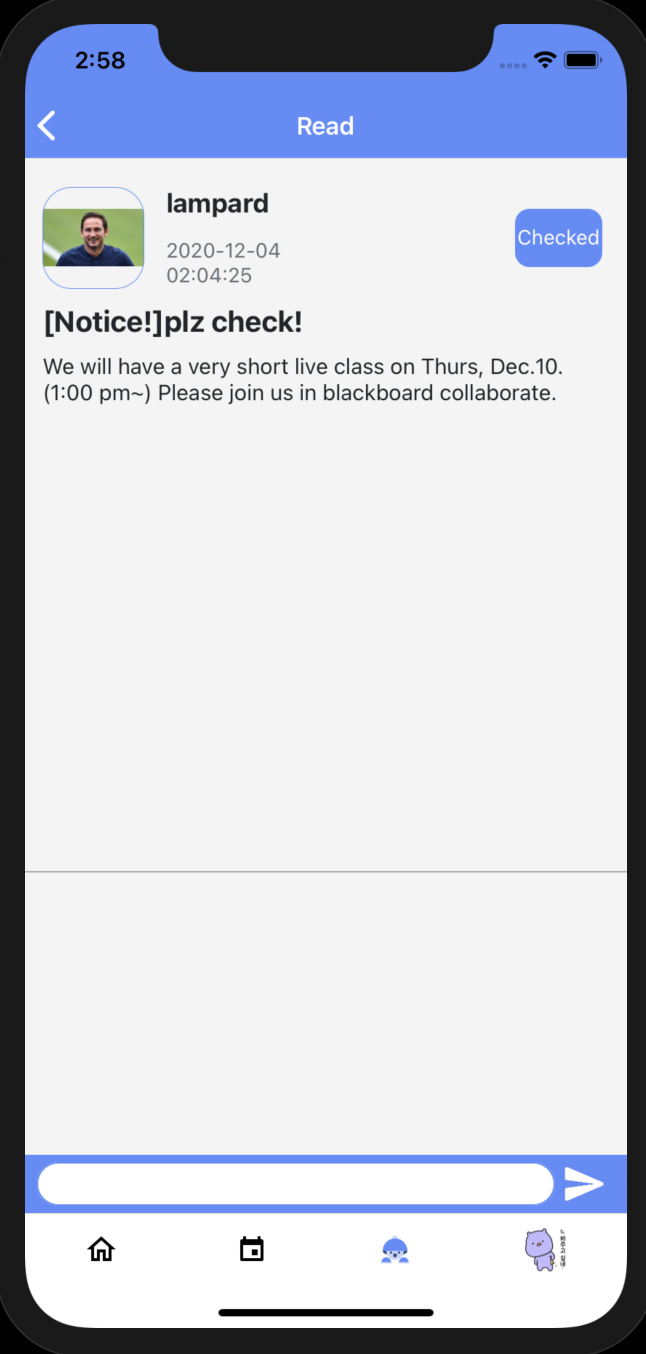
\includegraphics[width=4cm]{images/read5.png}
        \caption{Read Checked Screen}
        \label{fig:my_label}
    \end{figure}
    \begin{figure}[h]
        \centering
        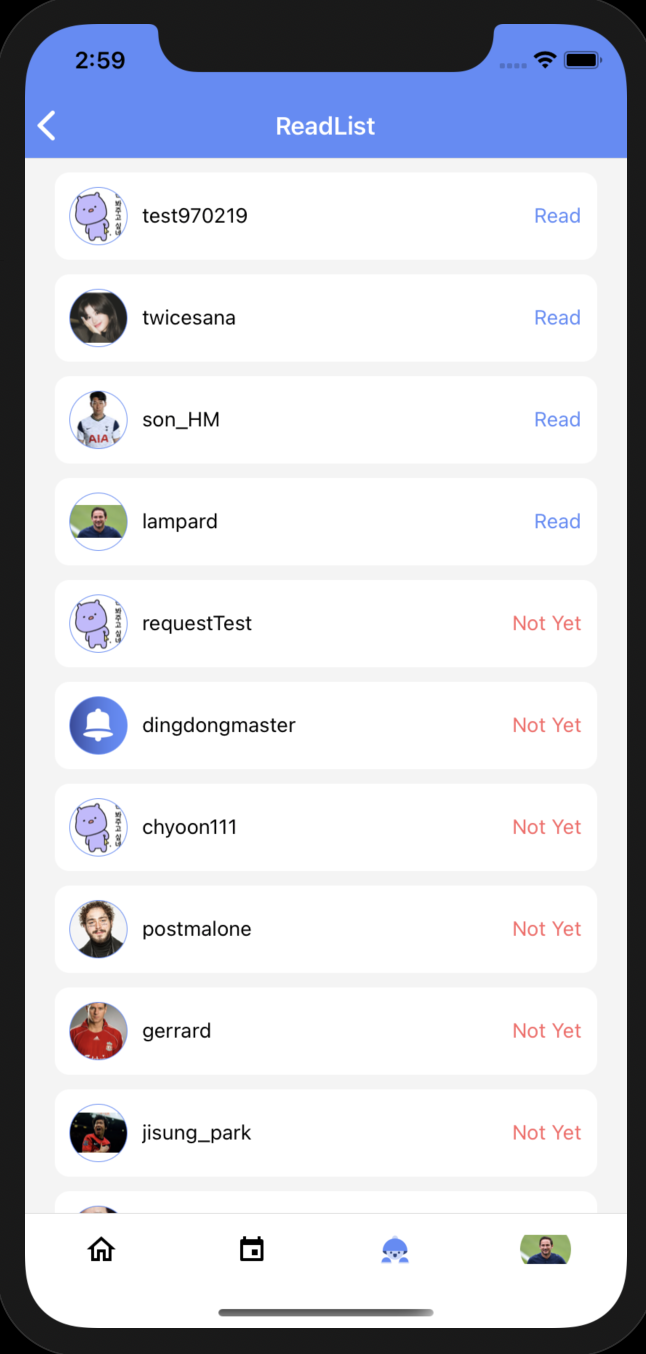
\includegraphics[width=4cm]{images/readlist.png}
        \caption{Read List Screen}
        \label{fig:my_label}
    \end{figure}
    \item Post Read Screen: In Post read screen, user can read the whole content of the post, and read comments. Also, comment input form is located at the bottom so that the user can type in new comments to the post. If the user is the writer of the post, and checked on check-read function on creation of the post, the check-list button will be displayed. Pressing on the button will navigate to Check Read List Screen. If the user is not the writer but the post has check-read function, the check-read button will be displayed. the text on the button will be ``Check Read". When pressing on it, the button will change to "Checked" and the user has successfully checked that he/she has read the post. 
    \begin{figure}[h]
        \centering
        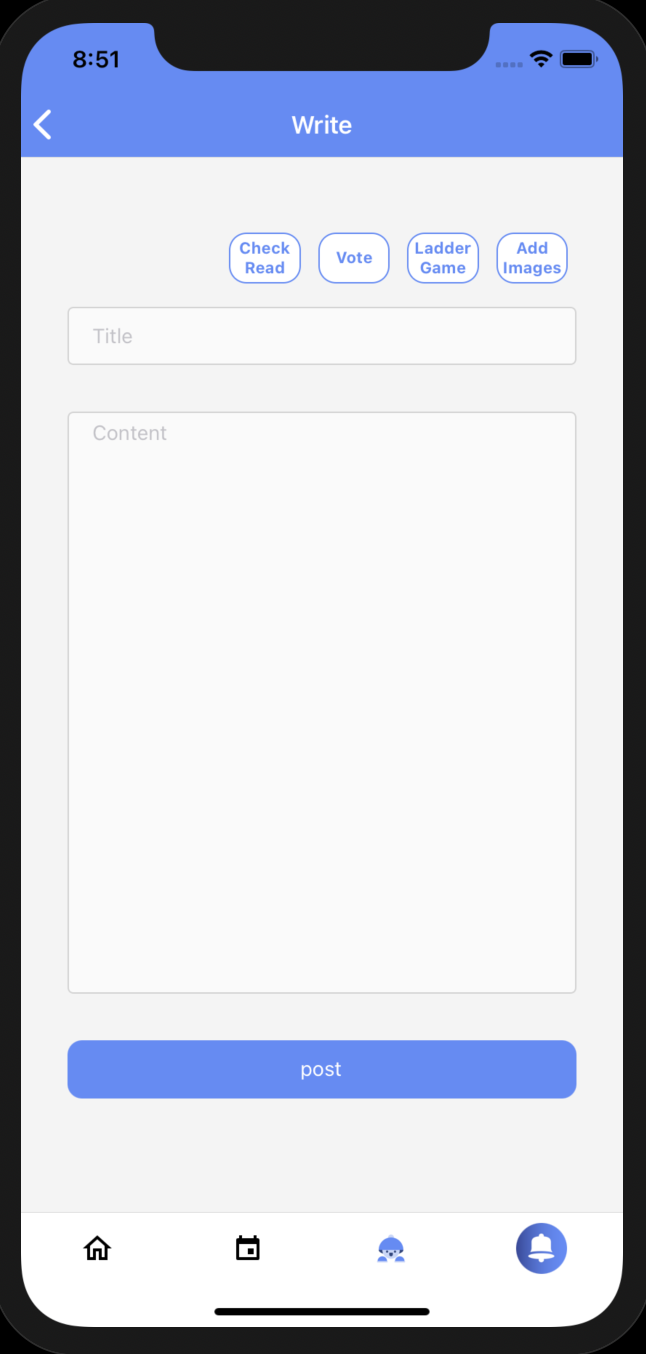
\includegraphics[width=4cm]{images/write1.png}
        \caption{Write Screen}
        \label{fig:my_label}
    \end{figure}
    \begin{figure}[h]
        \centering
        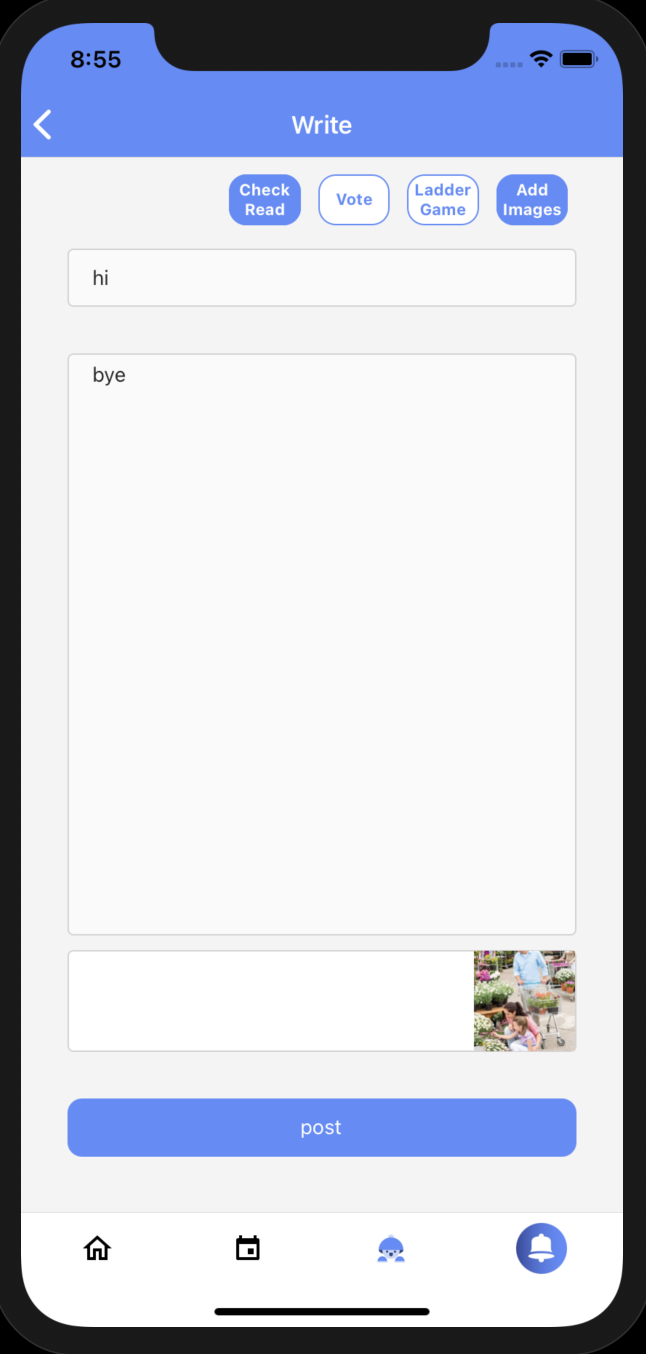
\includegraphics[width=4cm]{images/write2.png}
        \caption{Write Function highlight Screen}
        \label{fig:my_label}
    \end{figure}
    \item Post Write Screen: The post write screen is where users can create new posts. On the top of the screen, there are 4 functions. Check read is to decide whether to check if this post is going to be checking user read. Vote and Ladder game functions are not yet created. Add images are for adding images to the post. Up to 5 images can be posted.
    \begin{figure}[h]
        \centering
        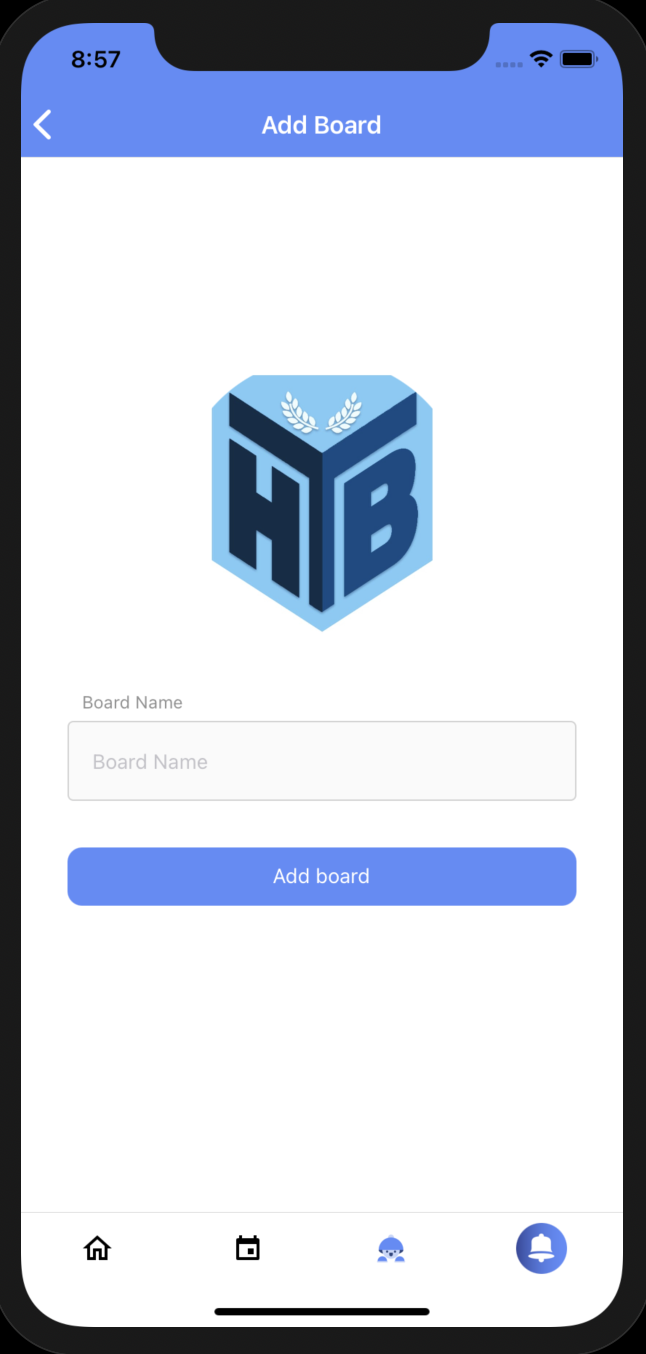
\includegraphics[width=4cm]{images/addboard.png}
        \caption{Add Board Screen}
        \label{fig:my_label}
    \end{figure}
    \item Add Board Screen: The Add Board screen is to add new board to the circle page. If receives the name of the board.
    \begin{figure}[h]
        \centering
        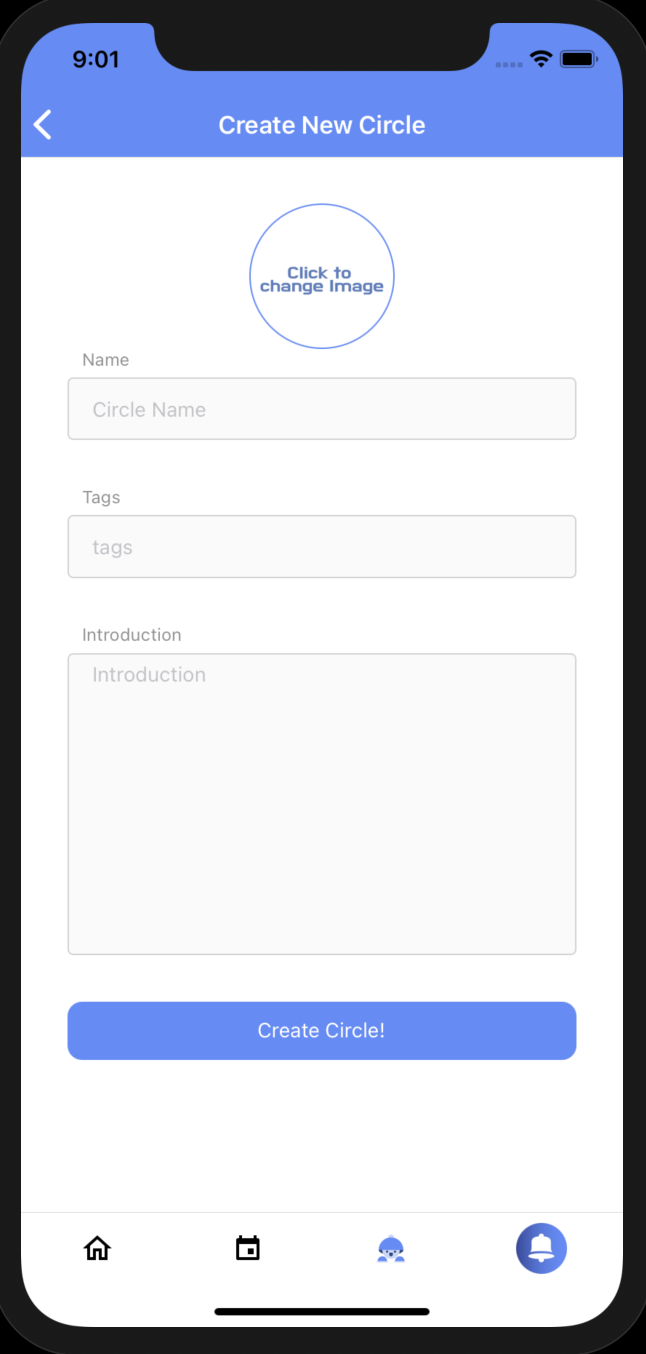
\includegraphics[width=4cm]{images/createnewcircle1.png}
        \caption{Create New Circle Screen}
        \label{fig:my_label}
    \end{figure}
    \begin{figure}[h]
        \centering
        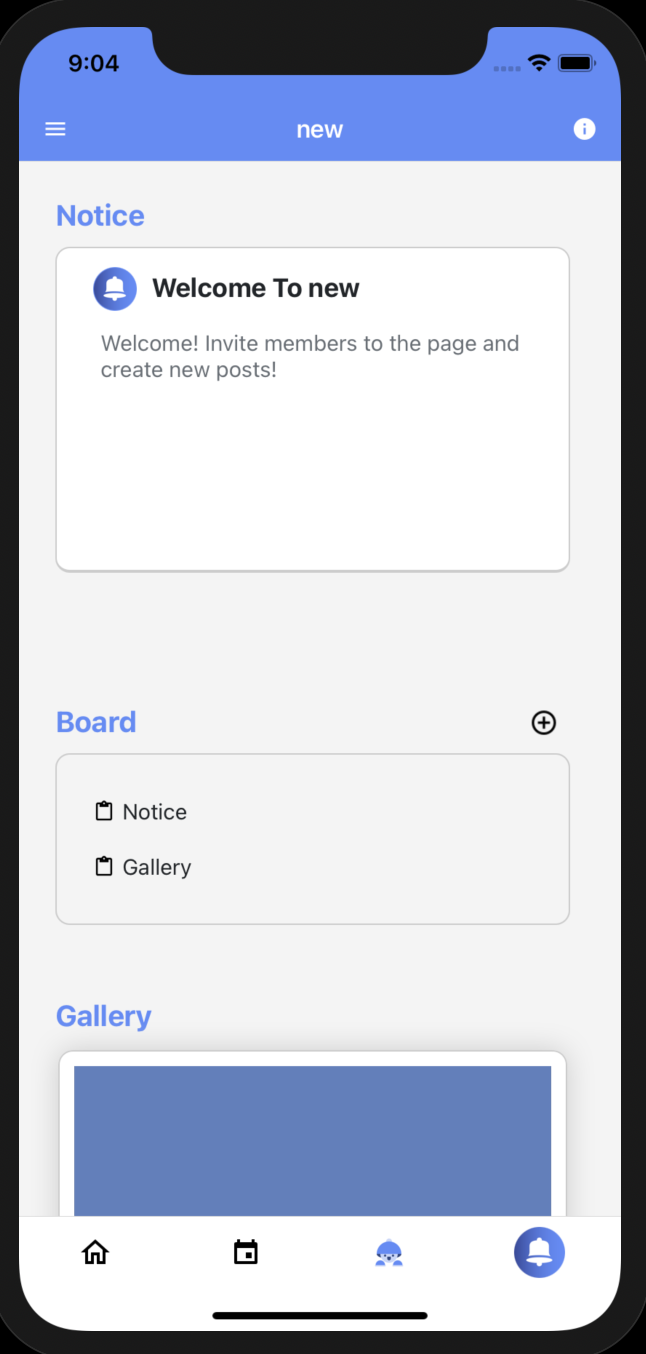
\includegraphics[width=4cm]{images/createnewcircle2.png}
        \caption{New Circle Screen}
        \label{fig:my_label}
    \end{figure}
    \item Create new Circle Screen: This page is for creating new circle pages. The form input receives the name, the tags and the explanation of the circle. The tags must be separated by space. If creation succeeds,it will navigate back. If fails, it will alert that it has failed. Newly created circle page has notice and gallery boards on default, and welcome post in the notice board.
    \begin{figure}[h]
        \centering
        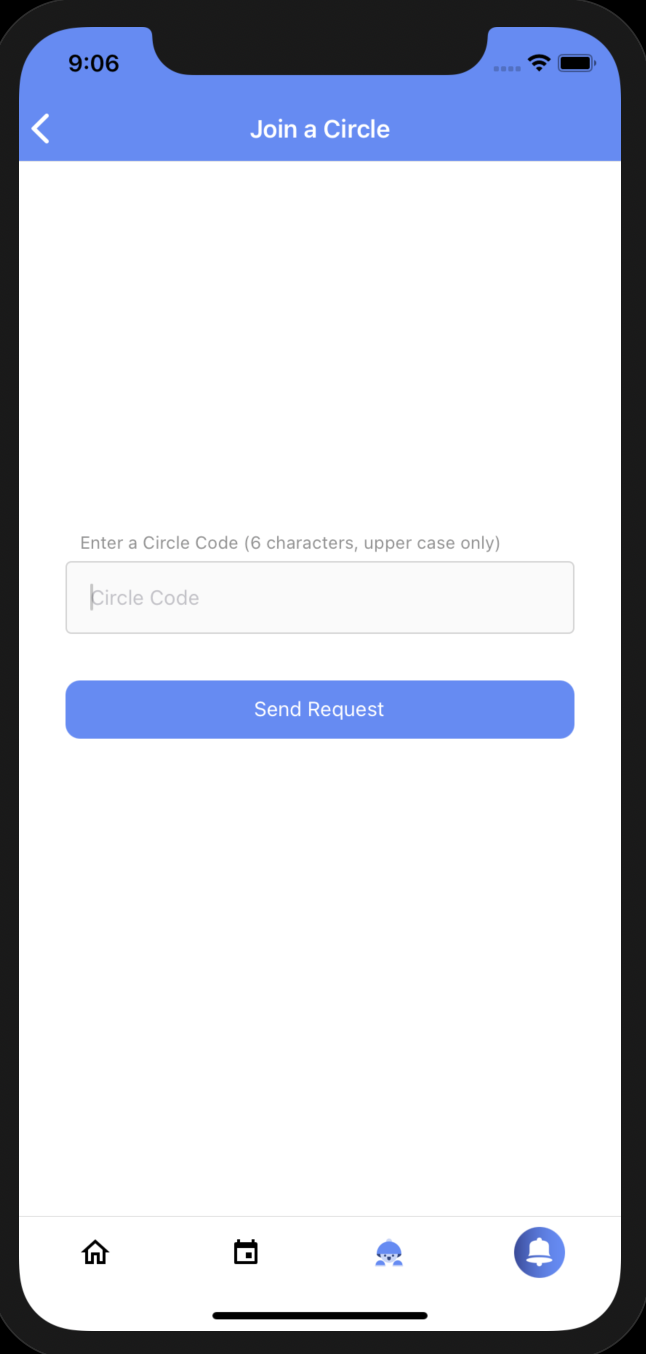
\includegraphics[width=4cm]{images/joinacircle1.png}
        \caption{Join a Circle Screen}
        \label{fig:my_label}
    \end{figure}
    \begin{figure}[h]
        \centering
        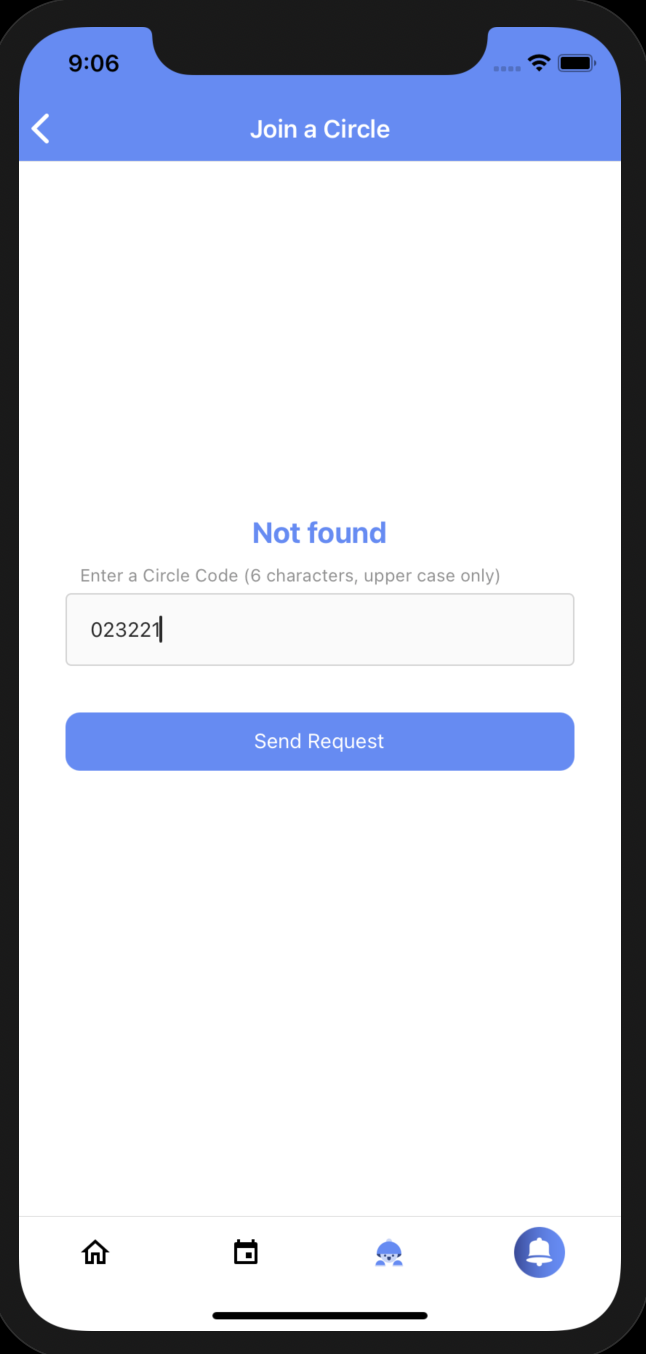
\includegraphics[width=4cm]{images/joinacircle2.png}
        \caption{Circle Not Found Screen}
        \label{fig:my_label}
    \end{figure}
    \item Join Circle Screen: Join Circle Screen is for joining a circle that you know the code of. Code is a random 6 digit code unique to each circles. Entering 6 digits will display the circle picture and name if it exists, or will show ``Not Found". 
    \begin{figure}[h]
        \centering
        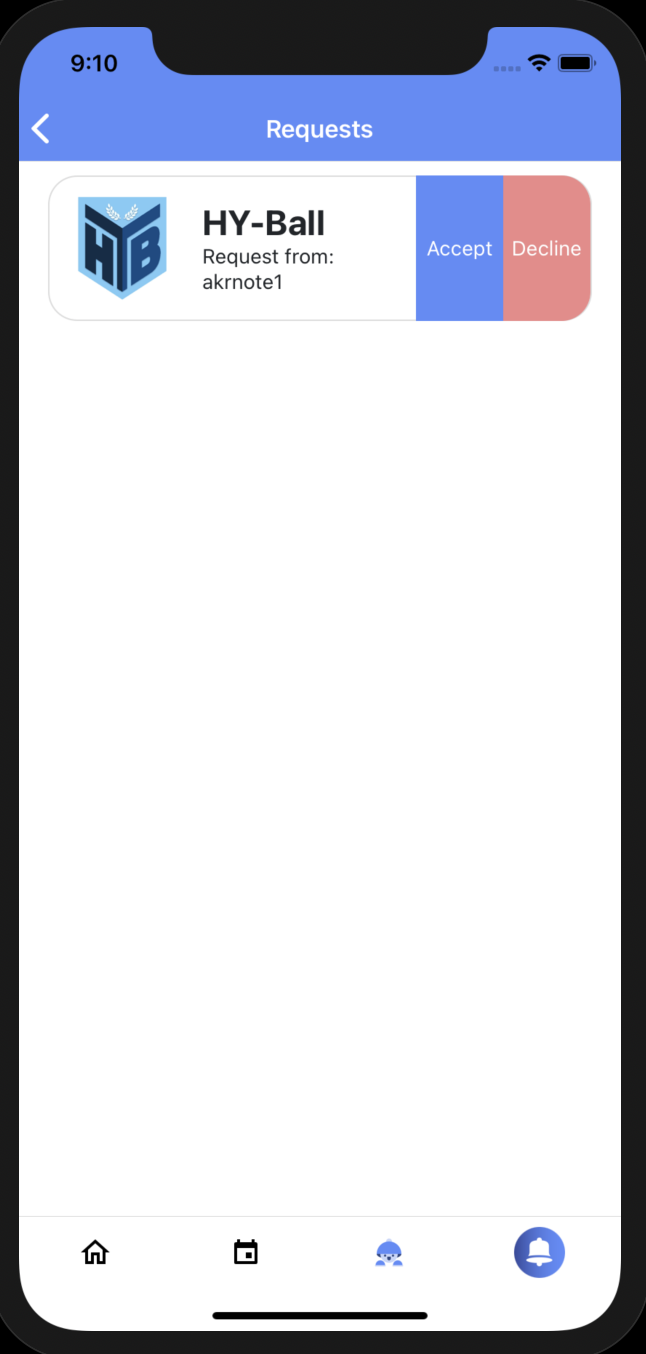
\includegraphics[width=4cm]{images/requests.png}
        \caption{Requests Screen}
        \label{fig:my_label}
    \end{figure}
    \item Request List Screen: The screen will display new requests to join a circle. Pressing on accept will accept new member to join. Pressing on decline will decline the request.
    \begin{figure}[h]
        \centering
        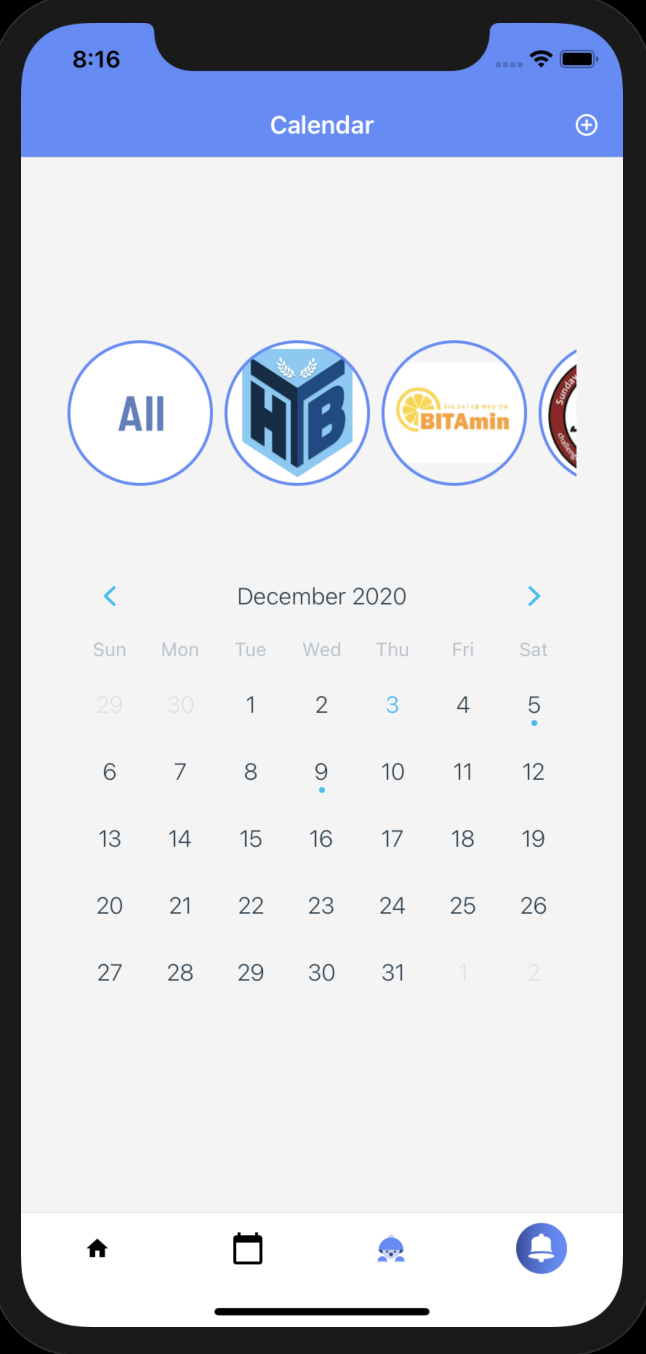
\includegraphics[width=4cm]{images/calendar1.png}
        \caption{Calendar Screen}
        \label{fig:my_label}
    \end{figure}
    \begin{figure}[h]
        \centering
        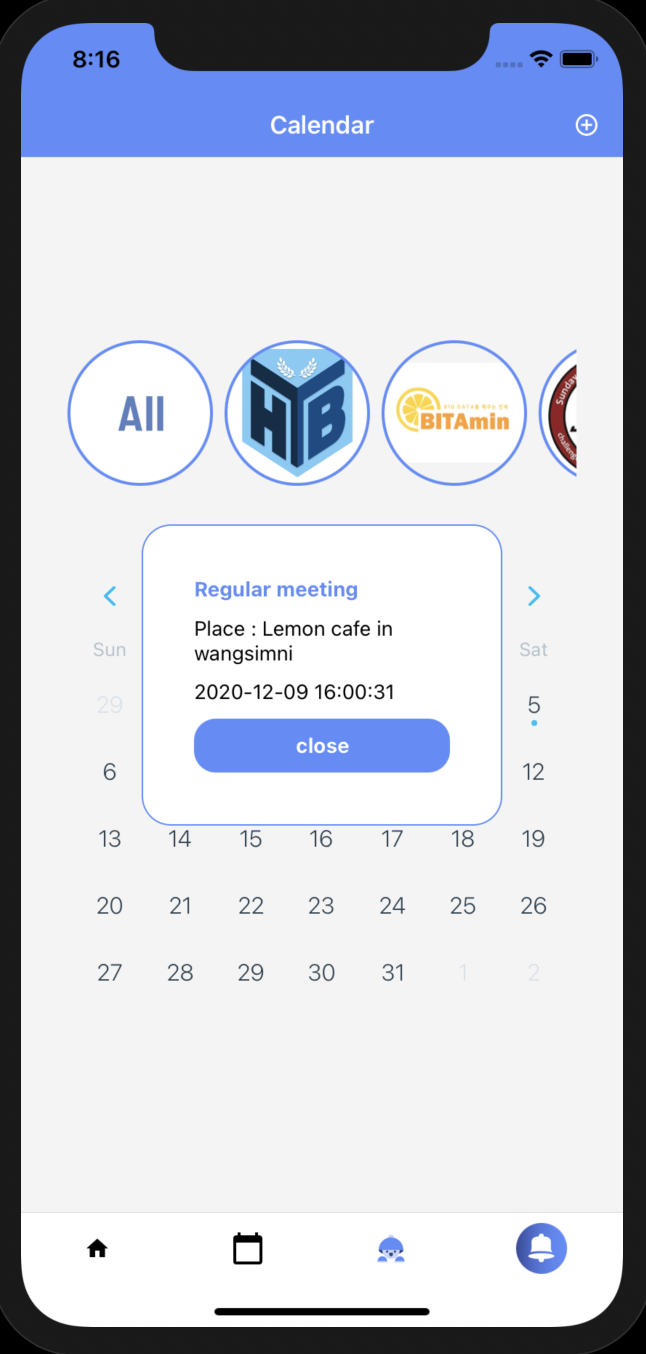
\includegraphics[width=4cm]{images/calendar2.png}
        \caption{Schedule Modal Screen}
        \label{fig:my_label}
    \end{figure}
    \item Calendar: This screen displays schedules of the circles. At first, all schedules of all circles will be shown. The date with a schedule will be marked with a dot. Pressing on the date will display the schedule details. On top, there is a list of circles. Pressing on each will display the schedules of that specific circle. On the header, there is a plus button which will navigate to add schedule screen.
    \begin{figure}[h]
        \centering
        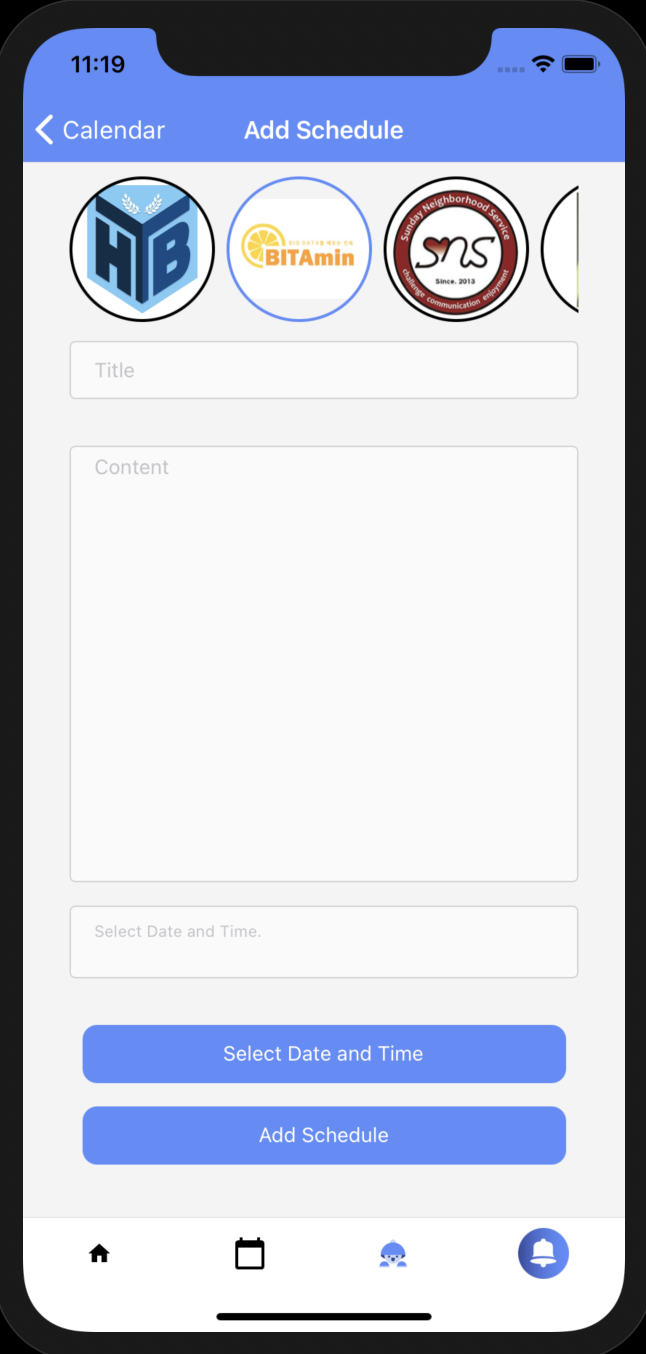
\includegraphics[width=4cm]{images/addschedule1.png}
        \caption{Add Schedule Screen}
        \label{fig:my_label}
    \end{figure}
    \begin{figure}[h]
        \centering
        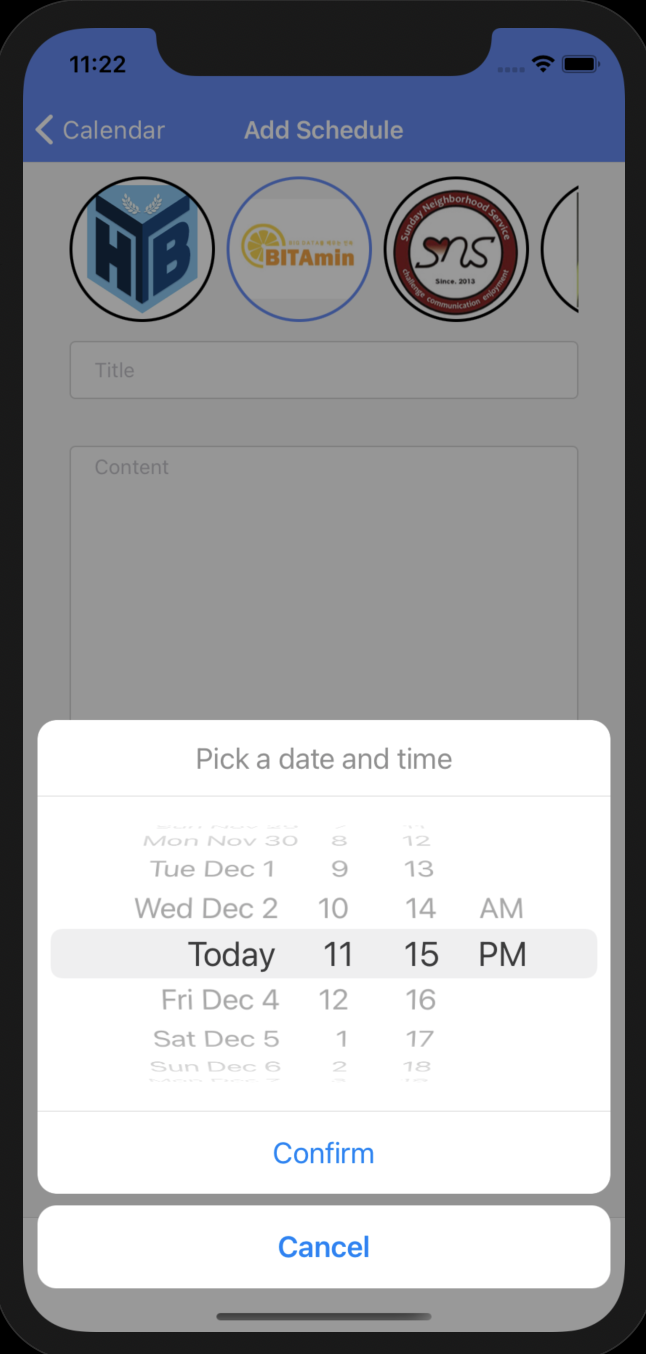
\includegraphics[width=4cm]{images/addschedule2.png}
        \caption{Pick a Date and Time Screen}
        \label{fig:my_label}
    \end{figure}
    \item Add Schedule Screen: This screen is for adding new schedule. On top, there is a list of circles that the user is admin of. Choose one circle and type in title and content and then select data and time to add a schedule.If success, it will navigate back to the Calendar screen and if not, it will alert that it has failed.
    \begin{figure}[h]
        \centering
        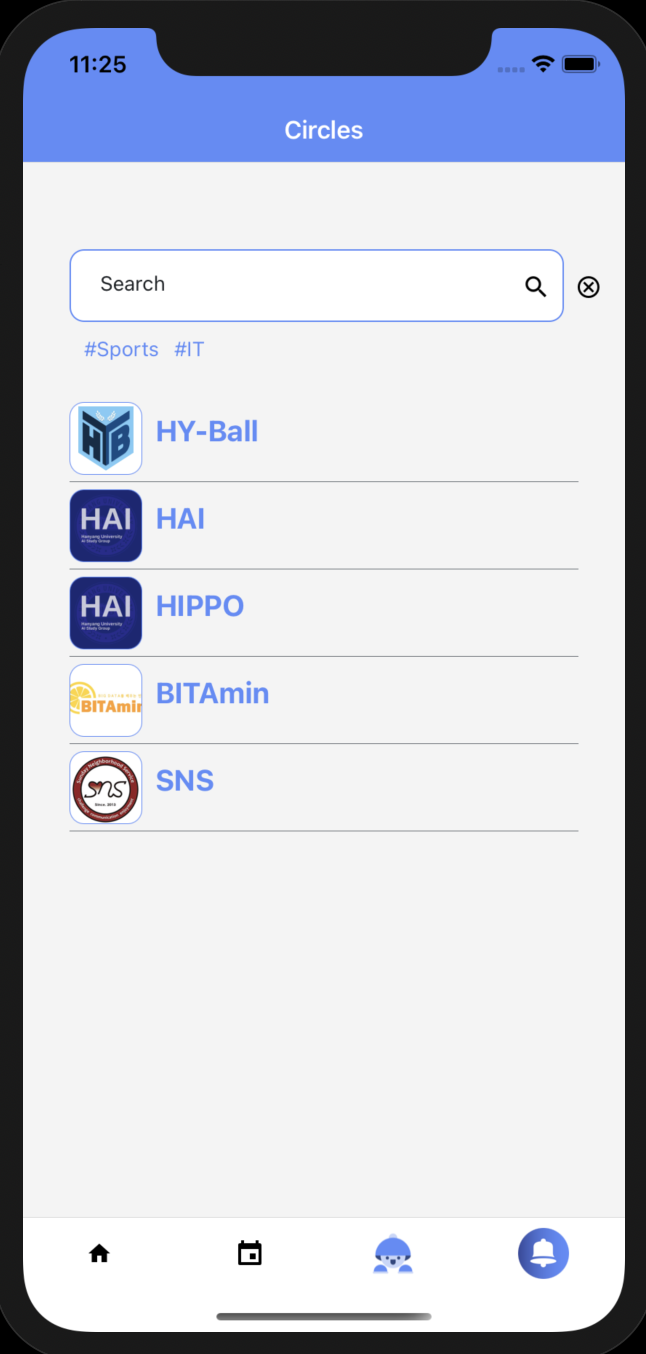
\includegraphics[width=4cm]{images/circles1.png}
        \caption{Circles Screen}
        \label{fig:my_label}
    \end{figure}
    \begin{figure}[h]
        \centering
        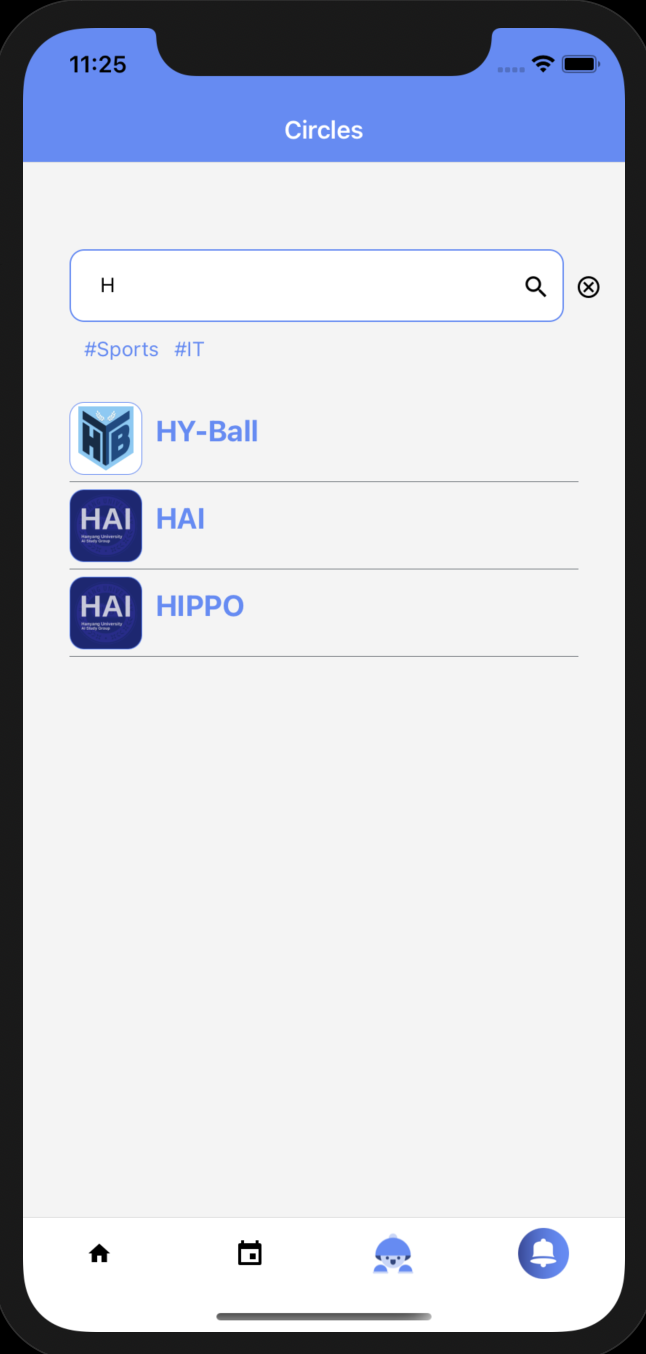
\includegraphics[width=4cm]{images/circles2.png}
        \caption{Circles Search Result Screen}
        \label{fig:my_label}
    \end{figure}
    \item Circles Screen: Circles screen is where list of circles and circle search is located. List will show 5 random circles to the user based on the user interest. Search is executed by typing in a name or tag of a circle that you want to search for. When searched, the list will change to the search result. To cancel a search, press the x button on the right side of the search bar. Pressing the searched circle will navigate to circle information screen.
    \begin{figure}[h]
        \centering
        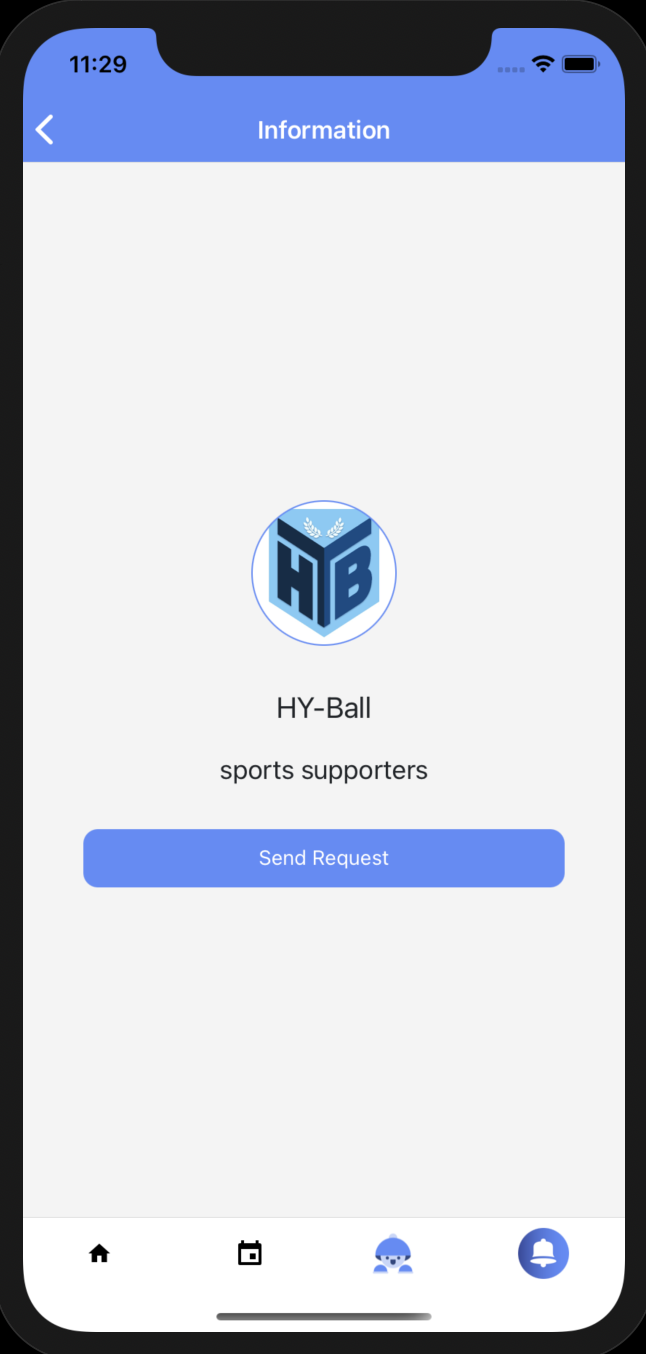
\includegraphics[width=4cm]{images/circlesinfo.png}
        \caption{Circles Information Screen}
        \label{fig:my_label}
    \end{figure}
    \item Circle Information Screen: This screen explains about the circle and allows the user to send join request.
    \begin{figure}[h]
        \centering
        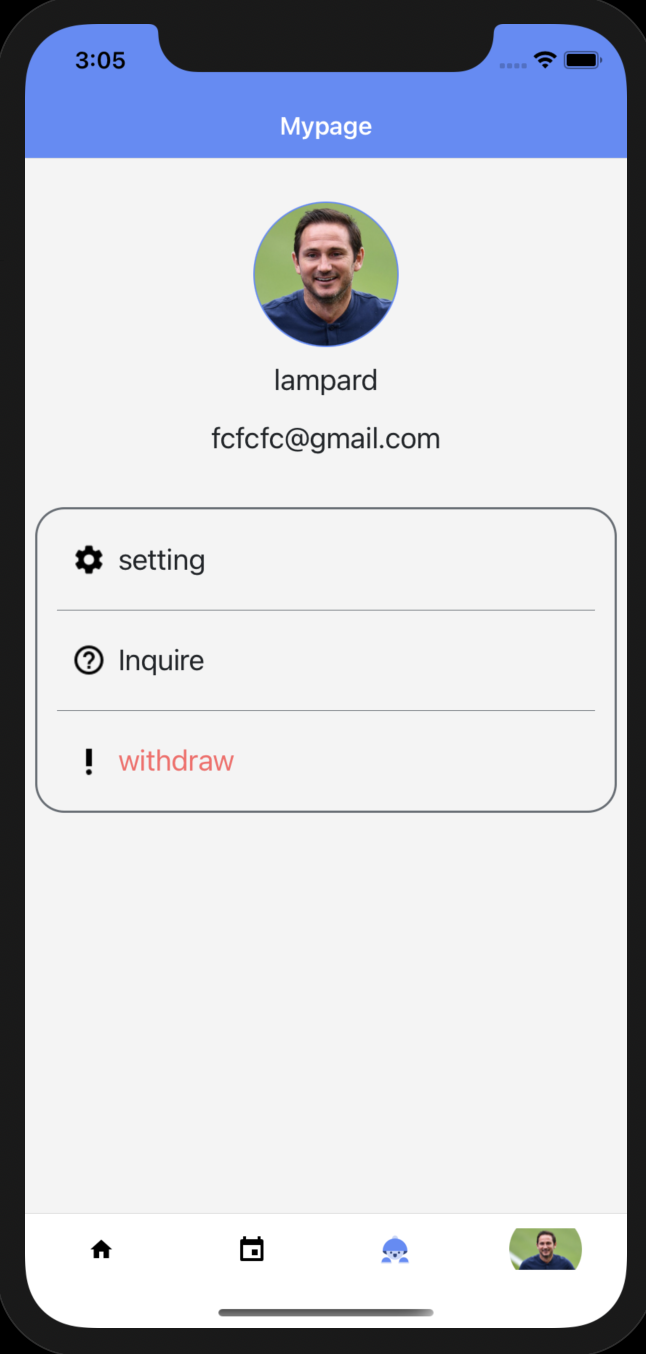
\includegraphics[width=4cm]{images/mypage.png}
        \caption{My Page Screen}
        \label{fig:my_label}
    \end{figure}
   
    \item My Page Screen: This screen is where user can modify its information, change settings, make inquires to the admins or to withdraw from dingdong. Pressing on user information will navigate to My page edit screen. Pressing on settings will open settings. Pressing Inquire Button will navigate to Inquire Screen. Pressing withdraw button will withdraw the user from dingdong, and navigate back to login screen.
     \begin{figure}[h]
        \centering
        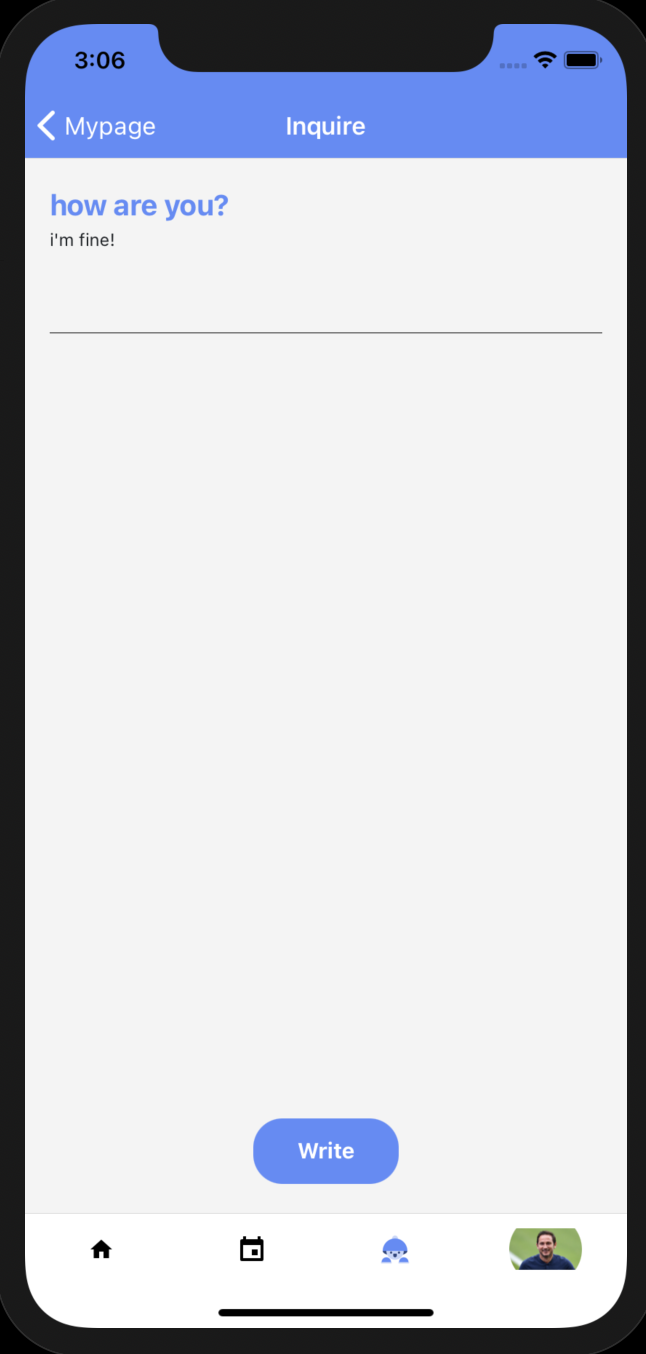
\includegraphics[width=4cm]{images/inquire.png}
        \caption{Inquire Screen}
        \label{fig:my_label}
    \end{figure}
    \iten Inquire Screen: This is where users can make inquires to the admin of dingdong. They can ask questions or suggest an idea by writing a new inquiry.
    \begin{figure}[h]
        \centering
        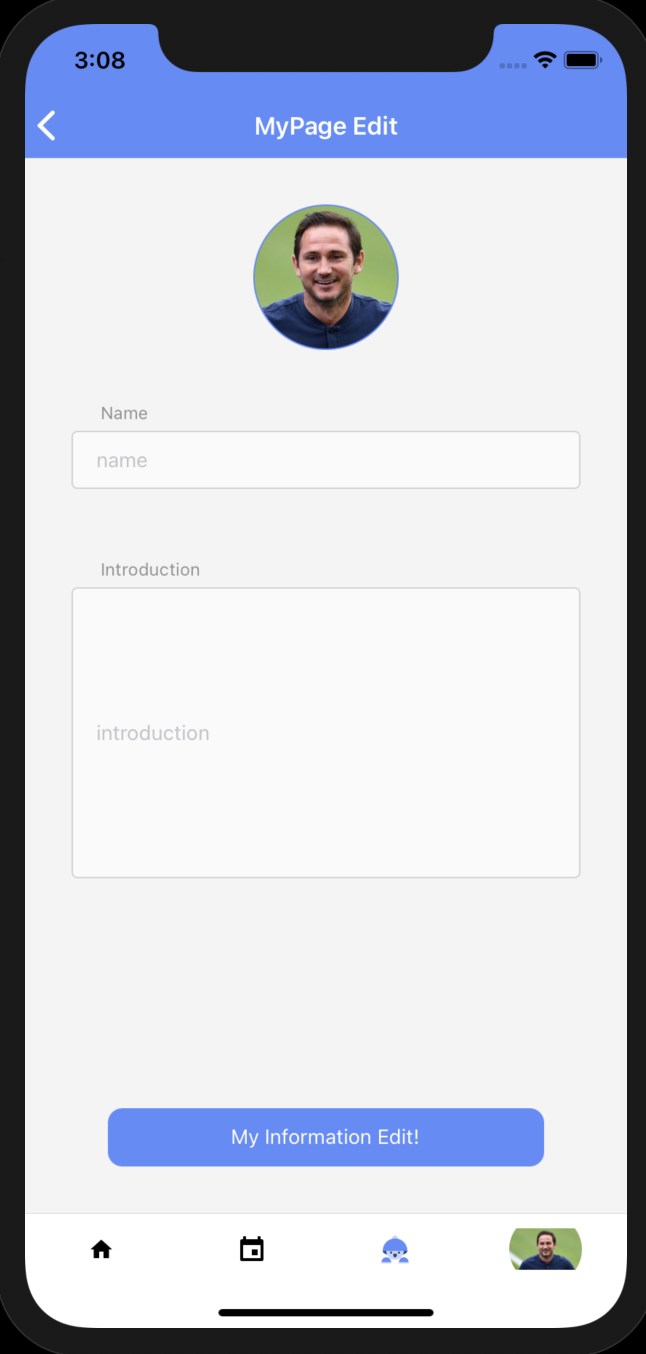
\includegraphics[width=4cm]{images/mypageedit.png}
        \caption{My Page Edit Screen}
        \label{fig:my_label}
    \end{figure}
    \item My page edit Screen: This screen is where users can change their information. Pressing on the profile picture will allow the user to select new profile image. The name and introduction can also be changed to a new one.
    
\end{enumerate}


\end{document}
